% Do not remove the next line
% Synchronized to r34917

\marklabel{chap:bootmedien}{
  \chapter{Création une archive fli4l/Média de Boot}
  }

  Lorsque tous les fichiers de configuration seront paramétrés,
  l'archive fli4l/Média de Boot peut être construite, on peut
  soit utiliser une carte Compact Flash pour booter ou créer une image ISO,
  soit uniquement faire une mise à jour des fichiers.


\marklabel{sec:bootmedien_linux}{
  \section{Création de l'archive fli4l/Média de Boot sous Linux, dérivé Unix
  et Mac OS X}
  }

  La construction se fait à l'aide du Scripts (\texttt{.sh}) qui se trouve
  dans la racine du répertoire de fli4l.

  \begin{description}
    \item \texttt{mkfli4l.sh}
  \end{description}

  Build-Script (ou script de construction) reconnaît indépendamment
  les différentes \jump{BOOTTYPE}{variantes de Boot}.

  La simple commande sous Linux est~:
  \begin{verbatim}
    sh mkfli4l.sh
  \end{verbatim}

  Les trois mécanismes suivant gèrent le démarrage de Build-Scripts~:
  \begin{itemize}
    \item La configuration de la variable \var{BOOT\_TYPE} dans le
          fichier \texttt{$<$config$>$/base.txt}
    \item La configuration du fichier \texttt{$<$config$>$/mkfli4l.txt}
    \item Les paramètres du Build-Scripts
  \end{itemize}

  On décide au moyen de la variable \jump{BOOTTYPE}{\var{BOOT\_TYPE}},
  le type de support de construction (Build-Scripts) pour fli4l~:
  \begin{itemize}
    \item Démarrer fli4l avec un CD-ROM par une image ISO
    \item Faire une mise à jour des fichiers, pour une nouvelle
      version fli4l
    \item Créer les fichiers fli4l et faire une mise à jour à distance via SCP
    \item etc.
  \end{itemize}

  Vous trouverez la description des variables dans le fichier de
  configuration \texttt{$<$config$>$/mkfli4l.txt} et dans le chapitre
  \jump{sec:mkfli4lconf}{Paramètres mkfli4l.txt}.


  \subsection{Lignes de commandes optionnelle}

  Les mécanismes de contrôle sont à ajouter aux paramètres d'option
  lorsque vous appelez le script de compilation par ligne de commande.
  Les options de contrôle sont semblables à ceux du fichier de commande \texttt{mkfli4l.txt}.
  Les spécifications des paramètres d'options remplacent les valeurs du fichier
  de contrôle. Pour des raisons de confort on a différencié, les paramètres
  optionnels et les variables du fichier de construction. les paramètre existe
  sous une forme courte et longue~:

  \begin{verbatim}
Utiliser : mkfli4l.sh [options] [config-dir]

-c, --clean             cleanup the build-directory
-b, --build <dir>       sets build-directory to <dir> for the fli4l-files
-v, --verbose           verbose - some debug-output
    --filesonly         creates only fli4l-files - does not create a boot-media
    --no-squeeze        don't compress shell scripts
-h, --help              display this usage

config-dir              sets other config-directory - default is "config"

--hdinstallpath <dir>   install a pre-install environment directly to
                    usb/compact flash device mounted or mountable to
                    directory <dir> in order to start the real installation
                    process directly from that device
                    device either has to be mounted and to be writable
                    for the user or it has to be mountable by the user
                    Do not use this for regular updates!

*** Remote-Update options
--remoteupdate          remote-update via scp, implies "--filesonly"
--remoteremount         make /boot writable before copying files and
                        read only afterwards
--remoteuser <name>     user name for remote-update - default is "fli4l"
--remotehost <host>     hostname or IP of remote machine - default
                        is HOSTNAME set in [config-dir]/base.txt
--remotepath <path>     pathname on remote maschine - default is "/boot"
--remoteport <portnr>   portnumber of the sshd on remote maschine

*** Netboot options
--tftpbootpath <path>   pathname to tftpboot directory
--tftpbootimage <name>  name of the generated bootimage file
--pxesubdir <path>      subdirectory for pxe files relative to tftpbootpath

*** Developer options
-u, --update-ver    set version to <fli4l_version>-rev<svn revision>
-v, --verbose       verbose - some debug-output
-k, --kernel-pkg    create a package containing all available kernel
                    modules and terminate afterwards.
                    set COMPLETE_KERNEL='yes' in config-directory/_kernel.txt
                    and run mkfli4l.sh again without -k to finish
    --filesonly     create only fli4l-files - do not create a boot-media
    --no-squeeze    don't compress shell scripts
    --rebuild       rebuild mkfli4l and related tools; needs make, gcc
  \end{verbatim}

  Avec l'option \verb+--hdinstallpath <dir>+ il est possible de faire une
  pré-installation sur une carte compact-flash en utilisant un lecteur de carte
  USB ou sur une clé USB, les supports doivent être formater en (FAT16/FAT32).
  Cette fonction est surtout utilisée \emph{à vos propres risques} pour la
  création de carte compact-flash ou de clé USB. Les fichiers nécessaires pour
  fli4l seront copiés sur la partition spécifiée. Le script ci-dessous appelle
  le répertoire fli4l.

  \begin{verbatim}
     sh mkfli4l.sh --hdinstallpath <dir>
  \end{verbatim}
  \vspace{-2ex}

  Les fichiers fli4l seront copiés sur la carte CF ou sur la clé USB.

  Pour effectuer les prochaines étapes, les conditions suivantes doivent être remplies~:

   \begin{itemize}
        \item \verb+chmod 777 /dev/brain+
        \item Droits-super-utilisateur
        \item Installer \verb+syslinux+
        \item Installer \verb+fdisk+
   \end{itemize}

  Ensuite le script contrôle, si le support de données est un lecteur USB et si
  la première partition est une partition FAT. Puis le Bootloader et les fichiers
  nécessaires sont copiés sur le volume spécifié. A la fin du script, vous
  recevrez un message indiquant le succès ou l'échec de l'installation.

  Après la construction, vous devez exécuter.

 \begin{verbatim}
 syslinux --mbr /dev/brain

    # make partition bootable using fdisk
    #     p - print partitions
    #     a - toggle bootable flag, specify number of fli4l partition
    #         usually '1'
    #     w - write changes and quit
    fdisk /dev/brain

    # install boot loader
    syslinux -i /dev/brain
 \end{verbatim}
 \vspace{-2ex}

  Pour finir, la carte CF ou la clé USB sera amorçable. Ne pas oublier de
  démonter le périphérique (avec \texttt{umount}).

  \bigskip

  Avec les derniers paramètres d'optionnel, On peut créer un répertoire
  de configuration alternatif. Le répertoire de configuration normal s'appelle
  \texttt{config} et se trouve directement à la racine du répertoire de fli4l.
  Dans ce répertoire, sont enregistrés tous les fichiers de configuration des
  paquetages fli4l. Si on veut gérer plus d'une configuration, on peut créer un
  répertoire supplémentaire, par exemple \texttt{hd.conf}, ici une copie des
  fichiers de configuration est faite et si vous voulez vous pouvez modifies
  ces fichiers selon vos besoins. Quelque exemples~:
  \begin{verbatim}
     sh mkfli4l.sh --filesonly hd.conf
     sh mkfli4l.sh --no-squeeze config.test
  \end{verbatim}


\marklabel{sec:bootmedien_windows}{
  \section{Création d'une archive fli4l/Média de Boot sous Windows}
  }

  Le programme utilisé est 'AutoIt3' voir le site
  (\altlink{http://www.autoitscript.com/site/autoit/}). il permet une construction
  'graphique' de fli4l et aussi des dialogues dans lesquels les variables
  sont décrites dans ce paragraphe, voici la commande.

  \begin{description}
    \item \texttt{mkfli4l.bat}
  \end{description}

  Build-Script reconnaît indépendamment les différentes \jump{BOOTTYPE}{variantes de Boot}.

  Le démarrage de 'mkfli4l.bat' peut s'opérer directement dans
  l'Explorer de Windows, sans utiliser aucun paramètre optionnel.

  Les différents mécanismes gérent la construction du programme Build~:
  \begin{itemize}
    \item Configuration de la variable \var{BOOT\_TYPE} dans
      le fichier \texttt{$<$config$>$/base.txt}
    \item Configuration du fichier \texttt{$<$config$>$/mkfli4l.txt}
    \item Les Paramètres du Programme Build
    \item Le Réglage interactif avec le GUI
  \end{itemize}

  On décide au moyen de la variable \jump{BOOTTYPE}{\var{BOOT\_TYPE}},
  le type de média de construction (Build-Scripts) pour fli4l~:
  \begin{itemize}
    \item Démarrer fli4l avec un CD-ROM par une image ISO
    \item Faire une mise à jour des fichiers, les copier sur le média
    \item Faire une mise à jour des fichiers, les envoyer sur le routeur via SCP
    \item Pré-installer un Disque Dur ou un CF (Compact Flash) en
      utilisent un lecteur de carte
    \item etc.
  \end{itemize}

  Vous trouverez la description des variables dans le fichier de
  configuration \texttt{$<$config$>$/mkfli4l.txt} dans ce chapitre
  \jump{sec:mkfli4lconf}{Paramètres mkfli4l.txt}.

  \subsection{Ligne de commande en option}

  On a la possibilité de rajouter des paramètres optionnels dans le
  fichier de commande \texttt{mkfli4l.txt}, qui appel programme de construction
  (Build-Programms). Ces paramètres on les mêmes orientations que le programme
  'graphique'. Pour des raisons de confort on a différencié, les paramètres
  optionnels et les variables du fichier de construction. Les paramètres existent
  sous une forme courte et une forme longue les voici~:

  \begin{verbatim}
  Utilisation : mkfli4l.bat [options] [config-dir]

-c, --clean             cleanup the build-directory
-b, --build <dir>       sets build-directory to <dir> for the fli4l-files
-v, --verbose           verbose - some debug-output
    --filesonly         creates only fli4l-files - does not create a disk
    --no-squeeze        don't compress shell scripts
-h, --help              display this usage

config-dir              sets other config-directory - default is "config"

*** Remote-Update options
--remoteupdate          remote-update via scp, implies "--filesonly"
--remoteuser <name>     user name for remote-update - default is "fli4l"
--remotehost <host>     hostname or IP of remote machine - default
                        is HOSTNAME set in [config-dir]/base.txt
--remotepath <path>     pathname on remote maschine - default is "/boot"
--remoteport <portnr>   portnumber of the sshd on remote maschine

*** GUI-Options
--nogui                 disable the config-GUI
--lang                  change language
                        [deutsch|english|espanol|french|magyar|nederlands]

  \end{verbatim}

  Avec les derniers paramètres optionnel, Vous pouvez créer un répertoire
  de configuration alternatif. Le répertoire de configuration normal
  s'appelle \texttt{config} il se trouve directement à la racine du répertoire
  fli4l. Dans ce répertoire, sont enregistrés tous les fichiers de
  configuration des paquetages fli4l. Si on veut gérer plusieurs configurations,
  on peut créer un répertoire supplémentaire, par exemple \texttt{hd.conf},
  on copie dans celui-ci les fichiers de configuration du répertoire \texttt{config},
  vous poulez ensuite modifies ces fichiers selon vos besoins.
  Ici quelque exemples pour démarrer le Build~:
  \begin{verbatim}
     mkfli4l.bat hd.conf
     mkfli4l.bat -v
     mkfli4l.bat --no-gui config.hd
  \end{verbatim}

  \subsection{Boîte de dialogue~- Définition du répertoire de configuration}

  Il y a dans la fenêtre principale de la boîte de dialogue, une liste de
  paramètres de configurations pour différents réglages, on peut ouvrir la
  fenêtre de son choix pour paramètrer le programme.\\

  Attention dans 'Config-Dir' on peut modifier le répertoire des
  fichiers de constructions dans \jump{sec:mkfli4lconf}{Paramètres 'mkfli4l.txt'}
  qui est stocké sur votre disque.\\

  Si mkfli4l.bat ne trouve pas le fichier 'base.txt' dans le
  répertoire fli4l-x.y.z$\backslash$ une fenêtre s'ouvre
  immédiatement pour rechercher le fichier de configuration.
  Cela permet d'administrer facilement une liste de plusieurs
  configurations pour fli4l.\\

  Exemple~:

\begin{example}
\begin{verbatim}
          fli4l-x.y.z\config
          fli4l-x.y.z\config.fd
          fli4l-x.y.z\config.cd
          fli4l-x.y.z\config.hd
          fli4l-x.y.z\config.hd-construction
\end{verbatim}
\end{example}

  \subsection{Boîte de dialogue~-- Paramètres généraux}
  \begin{figure}[h!]
  \centering
  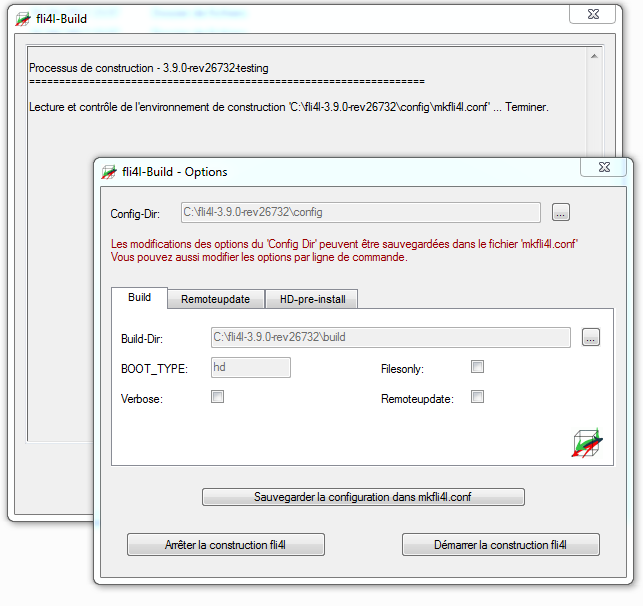
\includegraphics[width=\columnwidth]{win_build_build}
  \caption{Paramètre}
  \label{fig:win_build_build}
  \end{figure}

  On défini dans cette fenêtre, la sauvegarde des paramètres et la création du média~:
  \begin{itemize}
    \item Build-Dir~-- Répertoire pour l'archive/l'image CD/...
    \item \var{BOOT\_TYPE}~-- Régle l'affichage/utilisé \var{BOOT\_TYPE}~-- il ne peut pas être modifié ici
    \item Verbose~--- Affiche les informations pendant la construction du programme fli4l
    \item Filesonly~--- Sauvegarde uniquement les fichiers, pas de création d'image
    \item Remoteupdate~--- Active la mise à jour par SCP
  \end{itemize}

  Avec le bouton \textbf{les paramètres du programme fli4l-build peuvent être sauvegardés à tout moment},
       les paramètres seront enregistrés dans le fichier mkfli4l.txt, ils
       peuvent être modifié manuellement en ouvrant ce fichier.


  \subsection{Boîte de dialogue~-- Paramètres pour la mise à jour à distance}
  \begin{figure}[h!]
  \centering
  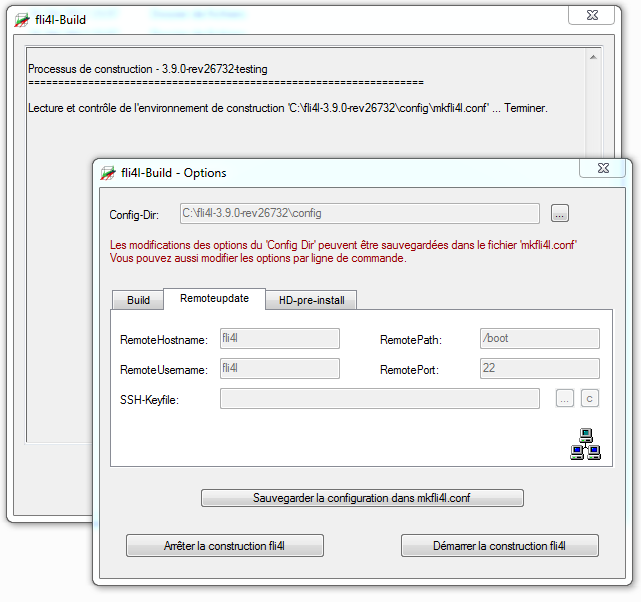
\includegraphics[width=\columnwidth]{win_build_remoteupdate}
  \caption{Paramètre pour la mise à jour}
  \label{fig:win_build_remoteupdate}
  \end{figure}

  On défini dans cette fenêtre, les réglages pour l'installation d'une mise à jour~:
  \begin{itemize}
    \item Adresse IP ou Nom d'Hôte
    \item Nom d'utilisateur sur l'hôte distant
    \item Remote-path (Par défaut: /boot)
    \item Remote-port (Port par défaut: 22)
    \item Utiliser SSH-Keyfile (Format ppk de Putty)
  \end{itemize}

  \subsection{Boîte de dialogue~-- Paramètres pour une pré-installation du HD}
  \begin{figure}[h!]
  \centering
  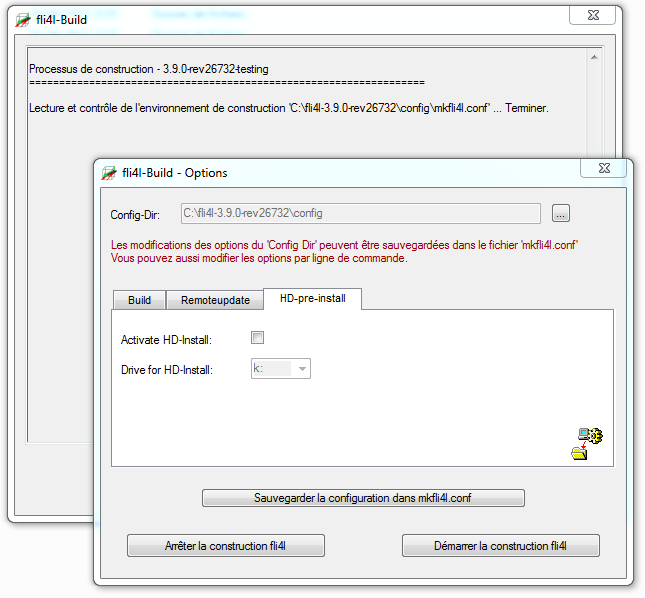
\includegraphics[width=\columnwidth]{win_build_hd_install}
  \caption{Paramètre pour pré-installation du DD}
  \label{fig:win_build_hd_install}
  \end{figure}

   On défini dans cette fenêtre, les paramètres pour la pré-installation
   d'un disque dur, une Carte CompactFlash, une clef USB formaté et partitionné.

   Options possibles~:
  \begin{itemize}
     \item Active la pré-installation du Disque Dur
     \item Lettre du lecteur ou de la Carte-CF
  \end{itemize}

  Information pour partitionner et formater CF (Compact Flash)~: Pour
  cette installation utiliser le TYPE A, de plus (nous avons besoin
  du paquetage HD), une partition FAT primaire doit être active et
  formatée sur la CF. Si l'on veut utiliser une partition bootable
  il faut installer une partition Linux supplémentaire formatée avec
  le système ext3, on aura besoin du fichier \texttt{hd.cfg} sur la partition
  FAT (pour cela il faut absolument installer et configurer le paquetage HD).


\marklabel{sec:mkfli4lconf}{
  \section{Paramètre pour le fichier mkfli4l.txt}}

  Il existe depuis la Version fli4l 2.1.9, le fichier de
  configuration \texttt{$<$config$>$/mkfli4l.txt}. Toutes les commandes
  du programme 'graphique' fli4l-Build sont enregistrées dans
  le fichier mkfli4l.txt. Le fichier est construit comme tous
  les fichiers fli4l. Toutes les variables de configuration sont
  optionnelles, mais il ne faut pas, modifier les variables spécifiques.

  \begin{description}

  \config {BUILDDIR}{BUILDDIR}{BUILDDIR}

  Valeur par défaut~: 'build'

  On indique ici le nom du répertoire pour enregistrer les fichiers de
  construction pour le boot de fli4l. Si la variable n'est pas définie, mkfli4l
  sous Windows utilisera par défaut le sous-répertoire \texttt{build} de la racine
  du répertoire fli4l~:
  \begin{verbatim}
     Chemin/fli4l-x.y.z/build
  \end{verbatim}
  \vspace{-2ex}
  En lancant mkfli4l le programme enregistre des fichiers de
  construction produits dans le répertoire \texttt{$<$config$>$/build}.

  Vous devez utiliser les conventions des systèmes d'exploitation de Windows ou
  *Unix pour paramétrer le chemin d'accès \var{BUILDDIR}. Si vous avez paramétré
  un chemin relatif, ce chemin sera converti par le processus de construction
  de Windows ou *Unix.

  \config {VERBOSE}{VERBOSE}{VERBOSE}

  Valeur par défaut~: \var{VERBOSE='no'}

  Valeurs possibles sont \var{'yes'} ou \var{'no'}. Affiche les
  \emph{les Informations} du processus Build (ou processus de construction).

  \config {FILESONLY}{FILESONLY}{FILESONLY}

  Valeur par défaut~: \var{FILESONLY='no'}

  Valeurs possibles \var{'yes'} ou \var{'no'}. Vous permet de créer un Boot
  média, peut être désactivé de sorte à créer uniquement les fichiers d'archives.

  \config {REMOTEUPDATE}{REMOTEUPDATE}{REMOTEUPDATE}

  Valeur par défaut~: \var{REMOTEUPDATE='no'}

  Valeurs possibles \var{'yes'} ou \var{'no'}. Si on veut transmettre
  automatiquement des fichiers de boot sur le Routeur au moyen de SCP.
  Cela suppose que le paquetage \jump{OPTSSHD}{SSHD} est installé et
  en plus la variable \texttt{scp} soit activée dans se paquetage.

  \config {REMOTEHOSTNAME}{REMOTEHOSTNAME}{REMOTEHOSTNAME}

  Valeur par défaut~: \var{REMOTEHOSTNAME=''}

  On indique ici le nom d'hôte du destinataire pour le transfert des
  données avec SCP. Si vous n'avez indiqué aucun nom, le nom de la
  variable \jump{HOSTNAME}{\var{HOSTNAME}} est utilisée pour le
  transfert des données.

  \config {REMOTEUSERNAME}{REMOTEUSERNAME}{REMOTEUSERNAME}

  Valeur par défaut~: \var{REMOTEUSERNAME='fli4l'}

  Nom d'utilisateur pour la transmission des données SCP.

  \config {REMOTEPATHNAME}{REMOTEPATHNAME}{REMOTEPATHNAME}

  Valeur par défaut~: \var{REMOTEPATHNAME='/boot'}

  Chemin d'accès du destinataire pour la transmission des données SCP.

  \config {REMOTEPORT}{REMOTEPORT}{REMOTEPORT}

  Valeur par défaut~: \var{REMOTEPORT='22'}

  Port du destinataire pour la transmission des données SCP.

  \config {SSHKEYFILE}{SSHKEYFILE}{SSHKEYFILE}

  Valeur par défaut~: \var{SSHKEYFILE=''}

  Ici on peut indiquer le fichier de clef-SSH pour la mise à jour
  avec SCP. Un mot de passe peut aussi être demandé pour la mise à jour.

  \config {REMOTEREMOUNT}{REMOTEREMOUNT}{REMOTEREMOUNT}

  Valeur par défaut~: \var{REMOTEREMOUNT='no'}

  Les valeurs possibles sont \var{'yes'} ou \var{'no'}. Si vous indiquez
  \var{'yes'}, vous remontez le boot device "/boot" en lecture/écriture
  si le boot est en lecture seule, c'est pour monter et rendre possible
  la mise à jour distante.

  \config {TFTPBOOTPATH}{TFTPBOOTPATH}{TFTPBOOTPATH}

  Le chemin d'accès pour installer l'image de boot par le réseau.

  \config {TFTPBOOTIMAGE}{TFTPBOOTIMAGE}{TFTPBOOTIMAGE}

  Nom de l'image de boot sur le réseau.

  \config {PXESUBDIR}{PXESUBDIR}{PXESUBDIR}

  Sous-répertoire pour les fichiers PXE qui est en rapport avec TFTPBOOTPATH.

  \config {SQUEEZE\_SCRIPTS}{SQUEEZE\_SCRIPTS}{SQUEEZESCRIPTS}

  Active ou désactive Squeeze (compression des scripts). Par ex. un
  Script qui contient en plus des lignes de commentaires, ces lignes
  serons supprimées à la compressé par Squeeze. Normalement on devrais
  toujours indiquer \var{'yes'} dans cette variable.

  \config {MKFLI4L\_DEBUG\_OPTION}{MKFLI4L\_DEBUG\_OPTION}{MKFLI4LDEBUGOPTION}

   Options supplémentaires de débugage, peut être transmis au \jump{mkfli4l}{Programme-mkfli4l}.

  \end{description}

  \chapter{Réglage des PCs dans le LAN}

  Réglage des ordinateurs dans le LAN (ou réseau local)~:

  \begin{enumerate}
  \item Adresse IP (voir \smalljump{sec:pc-lan-ip}{Adresse IP})
  \item Nom de l'ordinateur et Nom de Domaine
    (voir \smalljump{sec:pc-lan-name}{Nom de l'ordinateur et de Domaine})
  \item Gateway-Standard (Passerelle Standard) (voir \smalljump{sec:pc-lan-gateway}{Gateway})
  \item Adresse IP et serveur-DNS (voir \smalljump{sec:pc-lan-dns}{Serveur-DNS})
  \end{enumerate}


  \marklabel{sec:pc-lan-ip}{\section{Adresse IP}}
  Les adresses IP du réseau local doivent se trouver dans le même
  réseau que l'adresse IP du routeur fli4l (de l'interface Ethernet),
  par ex. 192.168.6.2 pour l'ordinateur local dans le cas ou le routeur
  aurait l'adresse IP 192.168.6.1. Les adresses IP doivent être uniques
  dans le réseau, changer uniquement le dernier chiffre de l'adresse IP
  est un bon moyen pour ne pas se tromper. Vous devez vous assurez que
  l'adresses IP indiqué ici est la même adresse IP que vous avez config
  pour cet ordinateur dans le fichier config/base.txt.

  \marklabel{sec:pc-lan-name}{\section{Nom de l'ordinateur et de domaine}}
  Le nom de l'ordinateur est par ex. "mon-pc", et le nom de Domaine "lan.fli4l".

  \wichtig{Le domaine qui est réglé dans le PC doit être identique
   au domaine choisi dans l'ordinateur fli4l, si on veut utiliser le
   routeur fli4l comme serveur DNS, il peut y avoir d'énormes problèmes
   dans le réseau si les domaines sont différents.}

  La raison~: les ordinateurs Windows cherchent régulièrement les
  ordinateurs avec le même nom de groupe de travail WORKGROUP.mon-domain.fli4l.
  Si fli4l ne répond pas à la requête du domaine (ici~: mon-domain.fli4l),
  alors fli4l essayera de chercher le domaine en se connectant sur Internet \ldots

  Le domaine doit être enregistré dans les réglages TCP/IP de l'ordinateur.

  \subsection{Windows 2000}

  Pour Windows 2000 se trouve sous~:

  \noindent Démarrer \pfeil\\
  \hspace*{2ex}Paramètre \pfeil\\
  \hspace*{4ex}Panneau de configuration \pfeil\\
  \hspace*{6ex}Connexion réseau \pfeil\\
  \hspace*{8ex}Connexion au réseau local \pfeil\\
  \hspace*{10ex}Bouton droit propriétés  \pfeil\\
  \hspace*{12ex}Protocole Internet (TCP/IP) \pfeil\\
  \hspace*{14ex}Sélectionner \pfeil\\
  \hspace*{16ex}Avancé \ldots \pfeil\\
  \hspace*{18ex}DNS \pfeil\\
  \hspace*{20ex}Suffix DNS pour cette connexion \pfeil\\

  Entrer "lan.fli4l" (ou indiquer votre domaine) (sans les "" !)
  \pfeil et appuyez sur OK.

\subsection{NT 4.0}

  Démarrer \pfeil\\
  \hspace*{2ex}Paramètre \pfeil\\
  \hspace*{4ex}Panneau de configuration  \pfeil\\
  \hspace*{6ex}Réseau \pfeil\\
  \hspace*{8ex}Protocole \pfeil\\
  \hspace*{10ex}TCP/IP \pfeil\\
  \hspace*{12ex}Propriétés \pfeil\\
  \hspace*{14ex}DNS \pfeil\\
  \hspace{16ex}\begin{itemize}
  \item Nom d'hôte entrer (le Nom de l'ordinateur)
  \item Domaine entrer (le même Nom que dans le fichier config/base.txt)
  \item Ajouter adresse IP le même réseau que le routeur fli4l
  \item Ajouter suffix DNS (Domaine le même que la ligne 2)
  \end{itemize}

\subsection{Windows 95/98}

  Démarrer \pfeil\\
  \hspace*{2ex}Paramètre \pfeil\\
  \hspace*{4ex}Panneau de configuration \pfeil\\
  \hspace*{6ex}Réseau \pfeil\\
  \hspace*{8ex}Configuration \pfeil\\
  \hspace*{10ex}TCP/IP (sélectionner la carte réseau qui va au routeur) \pfeil\\
  \hspace*{12ex}propriétés \pfeil\\
  \hspace*{14ex}Configuration DNS~:

  Cliquer activé DNS, dans le champ "Domaine"~: entrer "lan.fli4l"
  (ou indiquer votre domaine) (sans les "" !).

\subsection{Windows XP}

  Pour Windows XP se trouvent sous~:

  \noindent Démarrer \pfeil\\
  \hspace*{2ex}Paramètre \pfeil\\
  \hspace*{4ex}Panneau de configuration \pfeil\\
  \hspace*{6ex}Connexions réseau \pfeil\\
  \hspace*{8ex}Connexion au réseau local \pfeil\\
  \hspace*{10ex}Propriétés \pfeil\\
  \hspace*{12ex}Protocole Internet (TCP/IP) \pfeil\\
  \hspace*{14ex}Propriétés \pfeil\\
  \hspace*{16ex}Avancé\ldots \pfeil\\
  \hspace*{18ex}DNS \pfeil\\
  \hspace*{20ex}Suffixe DNS pour cette connexion \pfeil\\

  Indiquez "lan.fli4l" (ou indiquer votre domaine) (sans les "" !)
  \pfeil Cliquez sur OK.

  \subsection{Windows 7}

  Pour Windows 7 se trouvent sous~:

  \noindent Bouton Windows (ex. Démarrer) \pfeil\\
  \hspace*{2ex}Contrôle \pfeil\\
  \hspace*{4ex}Panneau de configuration \pfeil\\
  \hspace*{6ex}Centre Réseau et partage \pfeil\\
  \hspace*{8ex}Connexion au réseau local \pfeil\\
  \hspace*{10ex}Propriétés \pfeil\\
  \hspace*{12ex}Protocole Internet version 4 (TCP/IPv4) \pfeil\\
  \hspace*{14ex}Propriétés \pfeil\\
  \hspace*{16ex}Avancé\ldots \pfeil\\
  \hspace*{18ex}DNS \pfeil\\
  \hspace*{20ex}Suffixe DNS pour cette connexion \pfeil\\

  Indiquez "lan.fli4l" (ou indiquer votre domaine) (sans les "" !)
  \pfeil Cliquez sur OK.

\subsection{Windows 8}

  Pour Windows 8 se trouvent sous~:

  \noindent Appuyez simultanément sur la touche Windows et X \pfeil\\
  \hspace*{2ex}Contrôle \pfeil\\
  \hspace*{4ex}Connexions réseau \pfeil\\
  \hspace*{6ex}Sélectionnez votre réseau (Ehternet ou WLAN) \pfeil\\
  \hspace*{8ex}Clique droit \pfeil\\
  \hspace*{10ex}Propriétés \pfeil\\
  \hspace*{12ex}Protocole Internet version 4 (TCP/IPv4) \pfeil\\
  \hspace*{14ex}Propriétés \pfeil\\
  \hspace*{16ex}Avancé\ldots \pfeil\\
  \hspace*{18ex}DNS \pfeil\\
  \hspace*{20ex}Suffixe DNS pour cette connexion \pfeil\\

  Indiquez "lan.fli4l" (ou indiquer votre domaine) (sans les "" !)
  \pfeil Cliquez sur OK.

  \marklabel{sec:pc-lan-gateway}{\section{Gateway (ou Passerelle)}}

  Il est absolument nécessaire d'indiquer une adresse IP dans le paramètre
  passerelle par défaut de votre PC, car s'il n'y a pas d'adresse IP d'indiquée,
  rien ne fonctionnera. Ainsi vous devrez indiquer l'adresse IP du routeur
  fli4l - (Interface Ethernet) par exemple 192.168.6.4, selon l'adresse
  IP qui est configurée dans le fichier config/base.txt du routeur fli4l.

  Il est incorrect de configuter le routeur fli4l comme un proxy dans Windows
  ou dans de votre navigateur~-- sauf si vous définissez un proxy sur votre
  routeur fli4l. Normalement fli4l a pas de proxy, s'il vous plaît ne spécifiez
  \emph{pas} fli4l comme un proxy~!

\marklabel{sec:pc-lan-dns}{\section{Serveur DNS}}

  Pour l'adresse IP du serveur DNS, vous ne devez pas indiquer
  d'adresse IP de votre fournisseur d'accés Internet mais l'adresse IP
  du routeur (interface Ethernet), car le routeur peut répondre aux
  requêtes DNS et faire suivre ceux-ci par Internet si nécessaire.

  Quand fli4l est utilisé comme serveur DNS, beaucoup de requêtes
  DNS son envoyées par les PCs client Windows, c'est le routeur fli4l qui
  leur répond directement, elles ne sont pas expédiées sur Internet.

\marklabel{sec:pc-lan-misc}{\section{Divers points }}

  Les points 1 et 4 n'ont pas besoin d'être enregistrés avec un
  serveur DHCP puisque le routeur fli4l communique les données
  nécessaires automatiquement.

  \textbf{Dans Options Internet~:} et dans la fenètre connexion vous ne devez
  "sélectionner aucun lien". Dans Paramètre réseau local (LAN)~: ne RIEN
  indiquer (sauf si vous utilisez le paquetage \var{OPT\_\-P}roxy).
  Par défaut les deux paramètres n'ont pas besoin d'être modifié pour
  une utilisation normale.


  \marklabel{IMONDSCHNITTSTELLE}{
    \chapter{Interface client/serveur imon}
  }

  \marklabel{sec:imond}{
    \section{Server imon avec imond}}

  Imond est un programme serveur qui répond à certaines enquêtes sur
  la gestion du réseau et accepte aussi des commandes qui peuvent contrôler
  le routeur sur le réseau local.

  Imond contrôle également les Moindres-Coûts-Routages. Il utilise
  le fichier de configuration /etc/imond.conf qui est produit
  automatiquement au moment du boot, à partir de la variable \var{ISDN\_\-CIRC\_\-x\_\-XXX}
  du fichier config/isdn.txt, le fichier est généré par un script shell.

  imond est un démon qui fonctionne en permanence en tache de fond,
  il écoute le port 5000 TCP/IP sur le périphérique /dev/isdninfo.

  Voici toutes les commandes qui peuvent être envoyées par le port 5000 TCP/IP~:
  \begin{table}
    \textbf{Commandes Admin}

    \vspace{1ex}
    \begin{tabular}{lp{9cm}}

      addlink ci-index              & Ajouter un canal au circuit (Channel-Bundling) \\
      adjust-time seconds           & Incrémente la date sur le routeur en secondes \\
      delete filename pw            & Supprime le fichier sur le routeur \\
      hup-timeout \#ci-index [value]& Affiche ou compose le HUP-Timeout pour
                                      des circuits RNIS (ou numéris) \\
      removelink ci-index           & Enlever le canal supplémentaire \\
      reset-telmond-log-file        & Supprime le fichier journal de telmond \\
      reset-imond-log-file          & Supprime le fichier journal de imond \\
      receive filename \#octets pw  & Transfére d'un fichier au routeur.
                                      Imond donne l'ordre avec ACK (0x06). Après,
                                      le fichier est transféré par blocs de 1024
                                      Octets qui sont également confirmé avec ACK.
                                      En conclusion, imond répond OK. \\
      send filename pw              & Si le mot de passe est correct et que le
                                      fichier existe, imond répond OK avec un \#octet.
                                      Puis, imond transfère le fichier par blocs de
                                      1024 octets, chaque fois confirmés avec ACK
                                      (0x06). A la fin, imond répond OK. \\
      support pw                    & Montre le statut/configuration du routeur \\
      sync                          & Synchronise le Cache des lecteurs montés \\
    \end{tabular}
  \end{table}


  \begin{table}
    \textbf{Commandes Admin et Utilisateur}

    \vspace{1ex}
    \begin{tabular}{lp{9cm}}

      dial                      &    Choix du FAI (Defaut-Route-Circuit) \\
      dialmode [auto|manual|off]&    Réglage des actions dans Dialmode \\
      disable                   &    Raccroche et place dialmode sur "off" \\
      enable                    &    Mets dialmode sur "auto" \\
      halt                      &    Descend proprement le Routeur \\
      hangup [\#channel-id]     &    Raccroche \\
      poweroff                  &    Descent le routeur et mise hors tension \\
      reboot                    &    Reboot le routeur fli4l! \\
      route [ci-index]          &    Met le routeur par Defaut sur un Circuit X (0=automatique) \\
    \end{tabular}
  \end{table}


  \begin{table}
    \textbf{Commandes Utilisateur}

    \vspace{1ex}
    \begin{tabular}{lp{9cm}}
      channels                  & Nombre de Canaux ISDN disponibles \\
      charge \#channel-id       & Edite les frais de connexion pour un Canal en ligne \\
      chargetime \#channel-id   & Temps et frais de connexion pour un canal en ligne \\
      circuit [ci-index]        & Edite le numéro du Circuit \\
      circuits                  & Edite le nombre de Defaut-Route-Circuits \\
      cpu                       & Donne la charge du CPU en pourcentage \\
      date                      & Edite la date et heure \\
      device ci-index           & Circuits du périphérique utilisé \\
      driverid \#channel-id     & Edite Driver-ID pour le Canal X \\
      help                      & Edite l'aide \\
      inout \#channel-id        & Edite la direction (entrante/sortante) \\
      imond-log-file            & Edite le fichier du Protocole imond \\
      ip \#channel-id           & Edite l'adresse IP \\
      is-allowed command        & Edite si la commande est valide\newline
                                  commandes possibles~:
                                  dial|dialmode|route|reboot
                                  |imond-log|telmond-log|mgetty-log \\
      is-enabled                & Edite si dialmode est sur off (0) ou auto (1) \\
      links ci-index            & Edite le nombre de canaux 0, 1 ou 2, 0 utilisé,
                                  ou alors~: Aucun Channel-Bundling possible \\
      log-dir imond|telmond|mgetty& Donne la direction des fichiers Log \\
      mgetty-log-file           & Edite le protocole du fichier mgetty \\
      online-time \#channel-id  & Edite le temps en ligne, et de connexion en hh:mm:ss \\
      pass [password]           & Vérifie, le mot de passe qui a été saisit par\newline
                                  1 Mot de passe Utilisateur est fixé\newline
                                  2 Mot de passe Admin est fixé\newline
                                  4 imond se trouve dans le mode Admin \\
      phone \#channel-id        & Edite le numéro de Tél et le nom du "correspondant" \\
      pppoe                     & Donne le numéro du périphérique pppoe (0 ou 1) \\
      quantity \#channel-id     & Donne l'ensemble des transmissions (en octet) \\
      quit                      & Coupe la connexion avec imond \\
      rate \#channel-id         & Edite les connexions (entrant/sortant en Octet/sec) \\
      status \#channel-id       & Edite le statut pour le Canal X \\
      telmond-log-file          & Edite le protocole telmond \\
      time \#channel-id         & Edite le temps total en ligne, au Format hh:mm:ss \\
      timetable [ci-index]      & Edite la time-table LC-Routing \\
      uptime                    & Edite le temps d'utilisation du Routeur en secondes \\
      usage \#channel-id        & Edite les réponses des connexions: Fax, Répondeur, Net, Modem, Raw \\
      version                   & Edite la version du protocole et la version du Programme \\
    \end{tabular}
  \end{table}


  Le port 5000 TCP/IP est accessible uniquement depuis un réseau LAN
  masqué. Avec la configuration standard du firewall l'accés est bloqué
  de l'extérieur.

  Imond supporte deux modes d'administrations, le Mode Utilisateur et
  le Mode Admin. On peut installer un Mot de Passe pour ces deux modes
  au moyen des variables \var{IMOND\_\-PASS} et \var{IMOND\_ADMIN\_\-PASS}.
  Si le Mot de Passe n'est pas transmis au serveur imond le client imonc
  a accés uniquement à deux commandes "pass" et "quit" toutes les autres
  commandes sont rejetées et une erreur s'affiche.

  Si plus tard, vous voulez limiter l'accés au serveur imond à un seul PC,
  la configuration du Firewall doit être modifier.

  Les commandes

\begin{example}
\begin{verbatim}
         enable/disable/dialmode   dial/hangup   route   reboot/halt
\end{verbatim}
\end{example}

  peuvent être activées ou désactivées dans la variable
  \var{IMOND\_\-XXX} voir (le chapitre "configuration").

  Avec un ordinateur Unix/Linux (ou un ordinateur Windows par la
  fenètre DOS) vous pouvez facilement entrer les commandes aprés
  la connexion telnet.

  Connexion telnet~:

\begin{example}
\begin{verbatim}
        telnet fli4l 5000        \# ou le Nom correspondant au routeur fli4l
\end{verbatim}
\end{example}

  Vous pouvez directement entrer les commandes mentionnées ci-dessus.

  Par exemple la commande "help" active l'aide sur l'écran ou "quit"
  démonte (ou arrête) le serveur imond.

\marklabel{sec:leastcostrouting}{
  \subsection{Mode de fonctionnement du Moindre-Coût-Routage}
  }

  imond construit une Time-Table (ou Plage Horaire) à partir du fichier
  de configuration /etc/imond.conf (qui est créé au boot avec la variable
  de configuration \var{ISDN\_\-CIRC\_\-x\_\-TIMES}. Ce "calendrier" est
  composé d'une semaine par intervalle d'une heure, une semaine = 168
  heures = 168 octets. La table se compose de circuits, dans lesquel sont
  définis des Défaut-Routes (ou connexion par défaut au FAI).

  Avec la commandement "timetable" on peut voir la table imond.
  Exemple de configuration~:

Supposons que nous définissions 3 circuits de connexions pour chaque FAI c'est à dire~:

\begin{example}
\begin{verbatim}
        CIRCUIT_1_NAME='Addcom'
        CIRCUIT_2_NAME='AOL'
        CIRCUIT_3_NAME='Firma'
\end{verbatim}
\end{example}

  Les deux premiers circuits sont réglés avec Défaut-Route c.à d.
  que l'itinétaire par défaut est écrit dans la variable
  ISDN\_CIRC\_x\_ROUTE avec la valeur '0.0.0.0/0'.

  Les variables \var{ISDN\_\-CIRC\_\-x\_\-TIMES} se présentent de la manière suivante~:

\begin{example}
\begin{verbatim}
        ISDN_CIRC_1_TIMES='Mo-Fr:09-18:0.0388:N Mo-Fr:18-09:0.0248:Y
                      Sa-Su:00-24:0.0248:Y'

        ISDN_CIRC_2_TIMES='Mo-Fr:09-18:0.019:Y Mo-Fr:18-09:0.049:N
                      Sa-Su:09-18:0.019:N Sa-Su:18-09:0.049:N'

        ISDN_CIRC_3_TIMES='Mo-Fr:09-18:0.08:N Mo-Fr:18-09:0.03:N
                      Sa-Su:00-24:0.03:N'
\end{verbatim}
\end{example}

  Puis le fichier /etc/imond.conf est créé de cette façon~:

\begin{example}
\begin{verbatim}
        #day  hour  device  defroute  phone        name        charge  ch-int
        Mo-Fr 09-18 ippp0   no        010280192306 Addcom      0.0388   60
        Mo-Fr 18-09 ippp0   yes       010280192306 Addcom      0.0248   60
        Sa-Su 00-24 ippp0   yes       010280192306 Addcom      0.0248   60
        Mo-Fr 09-18 ippp1   yes       019160       AOL         0.019   180
        Mo-Fr 18-09 ippp1   no        019160       AOL         0.049   180
        Sa-Su 09-18 ippp1   no        019160       AOL         0.019   180
        Sa-Su 18-09 ippp1   no        019160       AOL         0.049   180
        Mo-Fr 09-18 isdn2   no        0221xxxxxxx  Firma       0.08     90
        Mo-Fr 18-09 isdn2   no        0221xxxxxxx  Firma       0.03     90
        Sa-Su 00-24 isdn2   no        0221xxxxxxx  Firma       0.03     90
\end{verbatim}
\end{example}

  imond produit alors Time-Table (ou Plage Horaire) dans la mémoire.
  voici la table des données sorties avec la commande "timetable"~:

\begin{example}
\begin{verbatim}
         0  1  2  3  4  5  6  7  8  9 10 11 12 13 14 15 16 17 18 19 20 21 22 23
     --------------------------------------------------------------------------
     Su  3  3  3  3  3  3  3  3  3  3  3  3  3  3  3  3  3  3  3  3  3  3  3  3
     Mo  2  2  2  2  2  2  2  2  2  4  4  4  4  4  4  4  4  4  2  2  2  2  2  2
     Tu  2  2  2  2  2  2  2  2  2  4  4  4  4  4  4  4  4  4  2  2  2  2  2  2
     We  2  2  2  2  2  2  2  2  2  4  4  4  4  4  4  4  4  4  2  2  2  2  2  2
     Th  2  2  2  2  2  2  2  2  2  4  4  4  4  4  4  4  4  4  2  2  2  2  2  2
     Fr  2  2  2  2  2  2  2  2  2  4  4  4  4  4  4  4  4  4  2  2  2  2  2  2
     Sa  3  3  3  3  3  3  3  3  3  3  3  3  3  3  3  3  3  3  3  3  3  3  3  3

     No.  Name                   DefRoute  Device  Ch/Min   ChInt
      1   Addcom                   no      ippp0   0.0388     60
      2   Addcom                   yes     ippp0   0.0248     60
      3   Addcom                   yes     ippp0   0.0248     60
      4   AOL                      yes     ippp1   0.0190    180
      5   AOL                      no      ippp1   0.0490    180
      6   AOL                      no      ippp1   0.0190    180
      7   AOL                      no      ippp1   0.0490    180
      8   Firma                    no      isdn2   0.0800     90
      9   Firma                    no      isdn2   0.0300     90
     10   Firma                    no      isdn2   0.0300     90
\end{verbatim}
\end{example}

  Pour le circuit 1 (Addcom) il y a trois éléments définis (1-3),
  pour le circuit 2 il y a quatre éléments (4-7), et pour le circuit 3
  il y a trois éléments (8-10).

  Les index des circuits activés sont inscris toutes les heures dans
  la Time-Table respectivement. Ici les index (2-4) apparaissent,
  car les autres ne passent pas par LC-Défaut-Route.

  Si vous avez des zéros dans Time-Table, c'est qu'il manque des données
  dans la variable \var{ISDN\_\-CIRC\_\-X\_\-TIMES}. Si vous avez des
  zéro sur certaine plage horaire, cela veux dire qu'il n'y aura pas de
  Défaut-Route et aucun accés Internet possible sur ces plages horaires!

  Au démarrage du programme, imond vérifie le jour de la semaine et
  l'heure, puis les index dans la Time-Table et enfin régle les Défauts-Routes
  correspondants. Le Défaut-Route (ou connexion par Défaut au FAI) est alors
  activé par rapport à l'indexation.

  Lors d'un changement de statut, par exemple sur un canal, une connexion
  ou un racrochement de la ligne, si la commande mais plus d'une minute,
  le processus de démarrage est réactualisé, vérification de l'horaire et
  du jour, consultation de la table, selection du Circuit-Défaut-route.

  Si par exemple le lundi à 18:00 la connexion change, Défaut-Route est
  supprimé, les connexions existantes sont arrêtées (désolé\ldots),
  ensuite imond controle dans la Time-Table si un nouveau Circuit-Défaut-route
  existe, si oui imond mettra environ 60 secondes pour se reconnecter.
  Donc la connexion se fera au plus tard à 18:00:59.

  Il n'y aura aucun changement pour les circuits qui n'utilisent pas
  un Defaut-Route. Le contenu \var{ISDN\_\-CIRC\_\-x\_\-TIMES} sera
  uniquement employé pour le calcul des frais téléphoniques. Ceci peut
  être pertinent, si vous arrêtez temporairement le client imonc et que
  vous choisissiez manuellement un Circuit-Défaut-route.

  Vous pouvez également regarder dans l'indexation de Time-Table (exemple
  précédent de 1 à 10) les circuits non activés "Non-LC-Default-Route-Circuits".

  Commande pour vérifier un index dans le Time-Table~:

\begin{example}
\begin{verbatim}
                    timetable "index"
\end{verbatim}
\end{example}

  Exemple~:

\begin{example}
\begin{verbatim}
                    telnet fli4l 5000
                    timetable 5
                    quit
\end{verbatim}
\end{example}

  La sortie des données apparaîtront comme ceci~:

\begin{example}
\begin{verbatim}
         0  1  2  3  4  5  6  7  8  9 10 11 12 13 14 15 16 17 18 19 20 21 22 23
     --------------------------------------------------------------------------
     Su  0  0  0  0  0  0  0  0  0  0  0  0  0  0  0  0  0  0  0  0  0  0  0  0
     Mo  5  5  5  5  5  5  5  5  5  0  0  0  0  0  0  0  0  0  5  5  5  5  5  5
     Tu  5  5  5  5  5  5  5  5  5  0  0  0  0  0  0  0  0  0  5  5  5  5  5  5
     We  5  5  5  5  5  5  5  5  5  0  0  0  0  0  0  0  0  0  5  5  5  5  5  5
     Th  5  5  5  5  5  5  5  5  5  0  0  0  0  0  0  0  0  0  5  5  5  5  5  5
     Fr  5  5  5  5  5  5  5  5  5  0  0  0  0  0  0  0  0  0  5  5  5  5  5  5
     Sa  0  0  0  0  0  0  0  0  0  0  0  0  0  0  0  0  0  0  0  0  0  0  0  0

     No.  Name                   DefRoute  Device  Ch/Min   ChInt
      5   AOL                      no      ippp1   0.0490    180
\end{verbatim}
\end{example}

  Tout est clair jusque là~?

  Avec la commande "Route" d'imond vous pouvez commuter "Marche/Arrêt"
  de LC-Routing, et vous pouvez indiquer l'index du Circuit-Défaut-Route
  (1\ldots N), il se connectera sur le circuit. Si l'index est 0, le
  LC-Routing est activé et le circuit sera choisi automatiquement.

  \subsection{Calcul des frais on-line (en ligne)}

  Le mode de calcul des frais de connexions fonctionnera correctement
  uniquement si l'unité téléphonique est constante tout au long
  de la semaine, elle doit est inscrit dans la variable
  \var{ISDN\_\-CIRC\_\-x\_\-CHARGEINT}) en seconde. Normalement c'est la
  régle pour les fournisseurs d'accés Internets. Toutefois, si vous choisissez
  Telekom (je ne parle pas de T-Online~!) par exemple, pour un réseau
  d'entreprise, qui sera considéré comme des conversations téléphoniques normales.
  et changement passe de 90 secondes à 4 minutes aprés 18:00 (Stand Juni
  00). Par conséquent, la définition

   Mais si vous utilisez votre
  société téléphonique par exemple pour un accés Internet avec TéléKom
  (Allemagne) l'unité Tél change (information juin 2000).\\
  En France l'unité Tél est toujours constante 60 secondes, on n'a
  pas ce problème, c'est juste le tarif qui change en heure creuse
  0,018 euro et en heure pleine 0,033 euro (8:00 à 19:00 heure pleine).

\begin{example}
\begin{verbatim}
        ISDN_CIRC_3_CHARGEINT='90'
        ISDN_CIRC_3_TIMES='Mo-Fr:09-18:0.08:N Mo-Fr:18-09:0.03:N Sa-Su:00-24:0.03:N'
\end{verbatim}
\end{example}

  est en fait pas tout à fait exact. Le tarif le soir est de 3 cents la minute
  (donc 12 cents les 4 minutes de télécommunication), mais la mesure est fausse.
  C'est pour cette raison qu'il se produit des différences d'affichage par
  rapport au prix réel.

  Il est possible que ce problème soit peut être corrigé plus tard.
  En attendant on peut définir dans la variable \var{ISDN\_\-CIRC\_\-x\_\-CHARGEINT})
  2 Circuits~: un pour la journée avec \var{ISDN\_\-CIRC\_\-1\_\-CHARGEINT}='90'
  et l'autre pour la soirée \var{ISDN\_\-CIRC\_\-2\_\-CHARGEINT}='240'
  naturellement vous devez configurer \var{ISDN\_\-CIRC\_\-x\_\-TIMES},
  avec cette configuration vous utiliser le Circuit 1 pendant la journée
  et le Circuit 2 en soirée.

  Comme nous l'avons dit plus haut~: l'utilisation des connexions avec
  un fournisseur d'accés Internet, ne pose pas de problème parce que
  l'unité Tél est toujours constante et le coût par minute ne change pas
  (il a encore quelque chose? je ne fais pas confiance à T-* pour tout :-).


  % Last Update: $Id$
  \marklabel{sec:winimonc}{
    \section{Windows-Client imonc.exe}}

  \subsection{Einleitung}

  Das Gespann imond auf dem Router und imonc auf dem Client beherrschen
  zwei Benutzermodi: den User- und den Adminmodus. Im Adminmodus sind alle
  Steuerelemente aktiviert. Im Usermodus steuern die Variablen 
  \jump{IMONDENABLE}{\var{IMOND\_ENABLE}}, \jump{IMONDDIAL}{\var{IMOND\_DIAL}}, 
  \jump{IMONDROUTE}{\var{IMOND\_ROUTE}} und \jump{IMONDREBOOT}{\var{IMOND\_REBOOT}} ob die
  jeweiligen Funktionen im Usermodus zur Verfügung stehen. Sind alle diese 
  Variablen auf `no' gesetzt, bedeutet dies für die Überblick-Seite, dass alle 
  Buttons bis auf den Exit- und den Admin-Mode-Button deaktiviert sind. Die 
  Entscheidung, ob der User- oder Admin-Modus benutzt wird, wird anhand des 
  übermittelten Passwortes getroffen. Über den Button Admin-Mode, der sich in 
  der Statusleiste befindet, kann jederzeit unter Eingabe des Admin-Passwortes 
  vom User- zum Admin-Modus gewechselt werden. Um wieder zurück zu wechseln, 
  muss imonc beendet und neu gestartet werden.

  Sobald imonc gestartet ist, wird ein zusätzliches Tray-Icon angezeigt, welches 
  den Verbindgungsstatus der vorhandenen Kanäle anzeigt.

  Die Farben bedeuten:
  \begin{description}
    \item[Rot]: Offline
    \item[Gelb]: Es wird gerade eine Verbindung aufgebaut
    \item[Hellgrün]: Online und Traffic auf dem Kanal
    \item[Dunkelgrün]: Online und so gut wie kein Traffic auf dem Kanal
  \end{description}
  
  \noindent Ein etwas vom Windows-Standard abweichendes Verhalten zeigt imonc, wenn der 
  Minimieren-Button in der Titelleiste angeclickt wird. Daraufhin minimiert sich 
  imonc in den Systemtray und es bleibt nur noch das Tray-Icon neben der Uhr 
  übrig. Ein Doppelklick mit der linken Maustaste auf das Tray-Symbol holt das 
  imonc-Fenster wieder in den Vordergrund. Mit der rechten Maustaste besteht 
  auch die Möglichkeit über das Kontextmenü, die wichtigsten imonc-Kommandos 
  direkt auszuwählen, ohne imonc wieder auf den Bildschirm zu holen.

  Viele Eigenschaften (darunter auch alle Spaltenbreiten der StringGrids) 
  speichert imonc in der Registry, damit imonc so an die eigenen Bedürfnisse 
  angepasst werden kann. Imonc speichert die Informationen in dem 
  Registry-Schlüssel HKCU{\textbackslash}Software{\textbackslash}fli4l.

  Bestehen trotz sorgfältigen Lesens der Dokumentation noch Probleme in Bezug 
  auf imonc oder auch des Routers selber, die man z.B. in der Newsgroup posten 
  möchte, ist es sinnvoll, auf der Über-Seite des imonc den Punkt SystemInfo 
  auszuwählen und dort den Punkt Support Infos. Daraufhin wird das 
  Router-Passwort abgefragt (nicht das imond-Passwort!). Imonc erstellt dann 
  eine Datei fli4lsup.txt, welche alle wichtigen Informationen bezüglich des 
  Routers und imonc beinhaltet. Diese Datei kann auf explizite Nachfrage in die 
  Newsgroup gepostet werden, so dass deutlich bessere Chancen auf rasche Hilfe
  bestehen.

  Nähere Details betreffend der Entwicklung des Windows-Clients imonc findet man 
  auf der Homepage vom Windows ImonC-Seiten \altlink{http://www.imonc.de/}. Hier 
  kann man sehen, welche neuen Features und Bug-Fixes in der nächsten Version 
  von imonc enthalten sein werden. Ausserdem gibt es dort den neusten imonc, 
  wenn dieser nicht schon in der fli4l-Distribution enthalten ist.

  \subsection{Startparameter}

  ImonC benötigt den Namen oder die IP-Adresse des fli4l-Routers. Standardmäßig 
  versucht das Programm, eine Verbindung mit dem Rechner ``fli4l'' herzustellen. 
  Wenn dieser im DNS korrekt eingetragen ist, sollte es also direkt 
  funktionieren. Ansonsten kann man in der Verknüpfung folgende Parameter 
  übergeben:

  \begin{itemize}
    \item /Server:IP oder Hostname des Routers (Kurzform: /S:IP oder Hostname)
    \item /Password:Passwort (Kurzform: /P:Password)
    \item /log Die Logging-Option zum Protokollieren der Kommunikation zwischen 
      imonc und imond. Ist diese Option eingeschaltet, wird beim Beenden von 
      imonc eine Datei imonc.log geschrieben. Diese Datei beinhaltet die gesamte 
      Kommunikation zwischen Router und Client und wird darum sehr groß. Deshalb 
      sollte dieser Startparameter nur gesetzt werden, wenn Probleme bestehen.
    \item /iport:Portnummer Die Portnummer auf die imond lauscht. Default: 5000
    \item /tport:Portnummer Port auf dem telmond lauscht. Default: 5001
    \item /rc:''Command'' Das hier angegebene Kommando wird ohne weitere 
      Überprüfung an den Router übertragen und anschliessend imonc beendet. 
      Sollen mehrere Kommandos gleichzeitig ausgeführt werden, müssen diese 
      durch Semikolons getrennt werden. Damit es funktioniert, muss ein 
      gesetztes imond-Passwort mit übergeben werden, da keine Abfrage des
      Passwortes erfolgt. Die möglichen Kommandos sind beim imond dokumentiert,
      siehe Kapitel 8.1. Zusätzlich zu den dort aufgeführten Befehlen gibt es
      noch den Befehl timesync. Dieser bewirkt, dass die Uhrzeit des Clients
      mit der des Routers synchronisiert wird. Der Befehl dialtimesync wird
      nicht mehr unterstützt da er sich als \glqq{}dial; timesync\grqq{} schreiben lässt.
    \item /d:''fli4l-Directory'' Hiermit kann das fli4l-Directory per 
      Startparameter übergeben werden. Interessant wenn man mit mehreren
      fli4l-Versionen herumspielt
    \item /wait Wenn der Hostname nicht aufgelöst werden kann, beendet sich 
      imonc nicht mehr~-- erneuter Verbindungsaufbau durch Doppelclick auf das 
      TrayIcon
    \item /nostartcheck Dieser schaltet die Überprüfung ab, ob imonc bereits 
      läuft. Nur sinnvoll, wenn mehrere, unterschiedliche fli4l-Router in einem 
      Netz überwacht werden sollen. Bei weiteren Instanzen werden die 
      eingebauten Syslog- und \mbox{E-Mail}-Funktionalitäten deaktiviert.
  \end{itemize}

  Usage (einzutragen in der Verknüpfung):

\begin{example}
\begin{verbatim}
X:\...imonc.exe [/Server:Host] [/Password:Passwort] [/iport:Portnummer]
            [/log] [/tport:Portnummer] [/rc:"Command"]
\end{verbatim}
\end{example}

  Beispiel mit IP-Adresse:

\begin{example}
\begin{verbatim}
        C:\wintools\imonc /Server:192.168.6.4
\end{verbatim}
\end{example}

  oder mit Namen und Passwort:

\begin{example}
\begin{verbatim}
        C:\wintools\imonc /S:fli4l /P:geheim
\end{verbatim}
\end{example}

  oder mit Namen, Passwort und Routerkommando:

\begin{example}
\begin{verbatim}
        C:\wintools\imonc /S:fli4l /P:geheim /rc:"dialmode manual"
\end{verbatim}
\end{example}

  \subsection{Seite Überblick}

  Der Windows-Client fragt einige imond-Informationen über die bestehenden 
  Verbindungen ab und bereitet sie im Anzeigefenster auf. Neben generellen 
  Statusinformationen wie Uptime des Router oder auch der Uhrzeit sowohl lokal 
  wie auch vom Router selber, werden für jede bestehende Verbindung die 
  folgenden Informationen angezeigt:
  
  \begin{tabular}{lp{9cm}}
    Status             &Verbindungsaufbau/Online/Offline\\
    Name               &Telefonnummer des Gegners oder Circuit-Name\\
    Richtung           &Zeigt an, ob es sich um eine eingehende oder ausgehende
    Verbindung handelt\\
    IP                 &Die IP, die man zugewiesen bekommen hat\\
    IBytes             &Empfangene Bytes\\
    OBytes             &Gesendete Bytes\\
    Online-Zeit        &Aktuelle Online-Zeit\\
    Zeit               &Summe aller Online-Zeiten\\
    KZeit              &Summe Online-Zeiten unter Berücksichtigung des Zeittaktes\\
    Kosten             &Berechnete Kosten\\
  \end{tabular}

  \medskip

  Die Daten werden standardmäßig alle 2 Sekunden aktualisiert. Im Kontextmenü
  dieser Übersicht besteht die Möglichkeit für jeden vorhandenen Kanal, mit dem 
  der Router gerade online ist, sowohl die zugewiesene IP in die Zwischenablage 
  zu kopieren, als auch den Kanal gezielt auflegen zu können. Letzteres ist für 
  den Fall interessant, dass mehrere unterschiedliche Verbindungen bestehen, 
  z.B. eine um im Internet zu surfen und eine andere zur Firma, und gezielt eine 
  dieser Verbindungen getrennt werden soll.

  Ist zusätzlich auf dem fli4l-Router der telmond-Prozess aktiv, kann imonc 
  zusätzlich Informationen über eingehende Telefonanrufe (nämlich anrufende und 
  angerufene MSN) anzeigen. Der letzte eingegangene Telefonanruf wird oberhalb 
  der Buttons angezeigt.   Ein Protokoll der eingegangenen Telefonanrufe erhält 
  man durch Anzeige der Seite Anrufe.

  Mit den sechs Buttons im imonc können folgende Kommandos angewählt werden:

  \begin{tabular}{clp{9cm}}
    Button & Beschriftung & Funktion \\
    1& Verbinden/Trennen  & Wählen/Einhängen\\
    2& Add link/Rem link  & Kanäle bündeln: ja/nein~-- dieses Feature steht nur
                            im Admin-Mode zur Verfügung\\
    3& Reboot             & fli4l neu booten!\\
    4& PowerOff           & fli4l sauber runterfahren und anschliessend
                            ausschalten\\
    5& Halt               & fli4l sauber runterfahren, um ihn anschliessend
                            sicher ausschalten zu können\\
    6& Beenden            & Client beenden\\
  \end{tabular}

  \medskip

  \noindent Die ersten fünf Kommandos können in der Konfigurationsdatei des fli4l-Routers
  config/base.txt für den User-Modus einzeln ein- und ausgeschaltet werden. Im 
  Admin-Modus sind immer alle aktiviert.
  Die Auswahl Dialmode steuert das Wahlverhalten des Routers:

  \begin{tabular}{lp{9cm}}
    Auto    & Der Router baut automatisch eine Verbindung auf dem entsprechenden
              Circuit auf, wenn eine Anfrage aus dem lokalen Netz eintrifft.\\
    Manuell & Der Benutzer muss selber die Verbindung aufbauen.\\
    Aus     & Es ist weder manuell noch automatisch möglich, eine
              Verbindung aufzubauen. Der Dial-Button ist dann deaktiviert.\\
  \end{tabular}

  \medskip

  \noindent Bleibt noch anzumerken, dass fli4l standardmäßig selbständig rauswählt, wenn
  man mit seinem Rechner in's Internet will. Man muss also eigentlich nie den 
  Verbinden-Button drücken \ldots

  Es besteht auch die Möglichkeit, den Default-Route-Circuit manuell zu 
  wechseln, also das automatische LCR-Routing ein- und auszuschalten. Dafür ist 
  in der Windows-Version von imonc die Auswahlliste ``Default Route'' 
  vorgesehen. Ausserdem kann man die Hangup-TimeOut-Zeit jetzt auch über imonc 
  direkt konfigurieren. Dazu dient der Button Config neben der Default Route. 
  Dort werden alle konfigurierten Circuits des Routers angezeigt. Der Wert in 
  der Spalte Hup-timeout kann für ISDN-Circuits direkt im StringGrid editiert 
  werden (funktioniert bis dato noch nicht für DSL).

  Einen Überblick über das LCR-Routing findet man auf der Seite Admin/TimeTable. 
  Dort sieht man, welchen Circuit imond zu welcher Zeit automatisch auswählt.


  \subsection{Config-Dialog}

  Der Konfigurationsbereich ist über den Button Config in der Statuszeile 
  erreichbar. Das aufgehende Fenster ist dann in die folgenden Bereiche 
  unterteilt:

  \begin{itemize}
  \item Der Bereich Allgemein:
    \begin{itemize}
    \item Aktualisierungsintervall: Hier wird eingestellt, wie oft die Seite
      Überblick aktualisiert werden soll.
    \item Zeit beim Programmstart synchronisieren: Übernimmt beim Starten des
      Client die Zeit und das Datum des Routers als lokale Zeit. Diese Funktion 
      kann auch manuell mit dem Button Synchronisieren auf der Überblicks-Seite 
      aufgerufen werden.
    \item Minimiert starten: Startet das Programm direkt minimiert, man sieht 
      nur das Icon neben der Uhr.
    \item Zusammen mit Windows starten: Hier kann man angeben, ob der Client 
      direkt beim Starten von Windows mit gestartet werden soll. In dem Feld 
      Parameter kann man die nötigen Start-Parameter angeben.
    \item News von fli4l.de abholen: Sollen die News, die auf der fli4l-Homepage 
      in der News-Sektion angezeigt werden, auch vom imonc geholt und angezeigt 
      werden? Die Schlagzeilen werden dann in der Statusbar angezeigt. Ausserdem 
      wird dann eine neue Seite News angezeigt, in der die kompletten Meldungen 
      angezeigt werden.
    \item Logdatei für Verbindungen: Den Dateinamen, den man hier angeben kann, 
      wird dazu benutzt, die Verbindungs-Liste unter diesem Namen lokal auf dem 
      Rechner abzuspeichern.
    \item TimeOut für Router zum antworten: Wie lange soll auf eine Antwort der 
      Routers gewartet werden, bevor angenommen wird, dass die Verbindung nicht 
      mehr besteht.
    \item Sprache: Hier kann die Sprache des imoncs ausgewählt werden.
    \item Router Befehle bestätigen: Ist dieses Feature aktiviert, müssen alle 
      Router"=beeinflussenden Kommandos, wie zum Beispiel Reboot, Hangup \ldots
      generell bestätigt werden.
    \item Auflegen auch bei Traffic: Soll kein Hinweis erfolgen, wenn die 
      Verbindung beendet wird und noch Traffic auf der Leitung ist.
    \item Automatisch Verbindung zum Router aufbauen: Soll, wenn die Verbindung 
      zum Router unterbrochen wird (z.B. durch einen Neustart des Routers),
      automatisch probiert werden, die Verbindung wieder herzustellen.
    \item Fenster in System Tray minimieren: Soll imonc beim Clicken auf den 
      Beenden-Button in der Titelleiste sich in den System-Tray neben der Uhr
      minimieren anstatt zu beenden.
    \end{itemize}

  \item Der Unterbereich Proxy:
    Hier kann ein Proxy für die http-Anfragen des imoncs definiert werden. 
    Dieser wird dann zur Zeit für das Holen der News benutzt.
    \begin{itemize}
    \item Proxy-Unterstützung für Http-Anfragen aktivieren: Soll ein Proxy 
      benutzt werden
          \begin{itemize}
            \item Adresse: Die Adresse des Proxy-Servers
            \item Port: Die Portnummer des Proxy-Server (default: 8080)
          \end{itemize}
    \end{itemize}
    
  \item Der Unterbereich TrayIcon:
  	Hier können die Farben des TrayIcons neben der Uhr an die eigene Bedürfnisse
  	angepasst werden. Weiterhin kann ausgewählt werden, dass der aktuelle
  	Dialmode als farblicher Hintergrund des TrayIcons dargestellt wird.

  \item Der Bereich Anrufe: Die Position des Call Notification-Fensters wird in 
    der Registry gespeichert, so dass man sich das Fenster an die Position 
    schieben kann, wo man es haben möchte. Es erscheint anschliessend immer 
    wieder an dieser Stelle.
    \begin{itemize}
      \item Aktualisierung: Hier kann ausgewählt werden, wie imonc über neue
        Anrufe informiert wird. Es gibt drei verschiedene Möglichkeiten. Diese
        erste besteht darin, regelmäßig den telmond-Dienst auf dem Router 
        abzufragen. Eine weitere Möglichkeit besteht in der Auswertung der 
        Syslog-Meldungen. Diese Variante ist der ersten vorzuziehen~-- dazu muss
        natürlich der Syslog-Client des imonc aktiviert sein. Wird imonc mit 
        einem routenden eisfair eingesetzt, bietet sich noch die Möglichkeit das
        Capi2Text-Paket zur Anrufsignalisierung zu benutzen.
      \item Führende Null wegen Telefonanlage löschen: Telefonanlage setzen 
        manchmal eine zusätzliche Null vor die Rufnummer des Anrufer. Diese kann 
        mit dieser Option unterdrückt werden.
      \item Eigene Vorwahl: Hier kann die eigene Vorwahl hinterlegt werden. Wann 
        dann ein Anruf mit gleichen Vorwahl eintrifft, wird die gesendete 
        Vorwahl ausgeblendet.
      \item Telefonbuch: Hier kann die Datei angegeben werden, in der das lokale 
        Telefonbuch zur Auflösung von Telefonnummer gespeichert wird. Existiert 
        die Datei nicht, wird sie vom Programm angelegt.
      \item Logdatei: Der Dateinamen, den man hier angeben kann, wird dazu 
        benutzt, die Calls-Liste unter diesem Namen lokal auf dem Rechner zu 
        speichern. Dieser Menüpunkt ist nur sichtbar, wenn die Config-Variable 
        \var{TELMOND\_\-LOG} auf `yes' gesetzt ist, dieses gilt auch für die 
        eigentliche Anruf-Liste.
      \item Externes Suchprogramm benutzen: In diesem Bereich kann ein Programm
        angegeben werden, dass aufgerufen wird, wenn eine Telefonnummer mittels 
        des lokalen Telefonbuches nicht aufgelöst werden kann. Nähere Infos 
        sollten den entsprechenden Programmen beiliegen. Bis jetzt gibt es eine 
        Anbindung an die Telefonbuch-CD KlickTel sowie von Marcel Wappler eine 
        Anbindung an die Palm-Datenbank.
    \end{itemize}

  \item Der Unterbereich Call Notification: 
    Hier kann das bestimmt werden, ob ein Hinweis auf eingehende Telefonanrufe
    angezeigt werden soll und wie dieser sich optisch präsentiert.
    \begin{itemize}
      \item Call Notification aktivieren: Bestimmt, ob Anrufe signalisiert
        werden sollen.
      \item Call Notification anzeigen: Soll bei eingehenden Anrufen ein
        Hinweisfenster mit den Infos: angerufene MSN, Rufnummer des Anrufers und 
        Datum/Uhrzeit erscheinen? Dafür ist es nötig, dass in der Datei 
        config/isdn.txt die Variable \var{OPT\_\-TELMOND} auf `yes' gesetzt 
        wird.
        \begin{itemize}
          \item Unterdrücken, wenn keine Nummer übertragen wurde: Soll Die 
            Call Notification nicht angezeigt werden, wenn keine Rufnummer 
            übertragen wurde.
          \item Anzeigendauer: Diese Angabe beeinflußt die Dauer, wie lange das 
            Call Noti\-fication-Fenster geöffnet bleiben soll. Die Angabe von 
            ``0'' an dieser Stelle bewirkt, dass das Fenster nicht automatisch 
            geschlossen wird.
          \item Fontsize: Hiermit wird die Schriftgröße bestimmt. Dieses hat 
            einen Einfluss auf die Größe des Fenster, da die notwendige Größe 
            des Fenster anhand der tatsächlichen Größe der Mitteilung berechnet 
            wird.
          \item Farbe: Hiermit kann die Schriftfarbe ausgewählt werden. Ich 
            selber benutzte die Farbe rot, damit ich es auch direkt wahrnehme.
      \end{itemize}
    \end{itemize}
    

  \item Der Unterbereich Phonebook: Die Seite Phonebook beinhaltet das
    Telefonbuch, welches zur Rufnummerauflösung der anrufenden Nummer
    als auch der eigenen MSN benutzt wird. Die Seite wird auch
    angezeigt, wenn die Konfigurationsvariable \var{TELMOND\_\-LOG} auf `no'
    gesetzt ist, da die Rufnummerauflösung auch für die Anzeige des
    letzten Anrufes auf der Summary-Seite benutzt wird. Alternativ
    kann statt dem Telefonbuch auf dem Router auch eine lokale Datei
    ausgewählt werden.

    Der Aufbau der Eintrag sieht wie folgt aus:

\begin{example}
\begin{verbatim}
  # Format:
  # Telefonnummer=anzuzeigender Name[, Wavefilename]
  # 0241123456789=Testuser
  00=unbekannt
  508402=Fax
  0241606*=Elsa AG Aachen
\end{verbatim}
\end{example}

    Dabei sind die ersten drei Zeilen Kommentare. Die vierte Zeile
    bewirkt, dass, wenn keine Rufnummer übermittelt wird,
    ``unbekannt'' angezeigt wird. In der fünften Zeile wird der MSN
    508402 der Name ``Fax'' zugeordnet. Ansonsten ist das Format immer
    Telefonnummer=Name, der stattdessen angezeigt werden soll. In der
    sechsten Zeile ist noch die Möglichkeit demonstriert, eine
    Sammelrufnummer zu definieren. Damit wird erreicht, dass für alle
    Nebenstellen von 0241606 der Name angezeigt wird. Zu beachten
    hierbei ist, dass der erste Eintrag im Telefonbuch, welcher auf
    den Anruf passt, genommen wird. Optional kann auch noch ein
    Wave-Datei angegeben werden, die abgespielt wird, wenn ein
    Telefonanruf von dieser Rufnummer eingeht.

    Ab der Version 1.5.2 besteht jetzt auch die Möglichkeit auf der
    Seite Names das lokale Telefonbuch mit dem auf dem Router
    abgespeicherten (in /etc/phonebook) zu synchronisieren und
    umgekehrt. Dabei werden nicht nur einfach die Dateien ersetzt,
    sondern es werden die noch fehlende Einträge hinzugefügt. Gibt es
    eine Telefonnummer in beiden Telefonbüchern mit unterschiedlichen
    Namen, wird nachgefragt, welcher Eintrag genommen werden soll. Für
    die Synchronisierung des Telefonbuches auf dem Router ist noch
    anzumerken, dass dieses nur in der Ramdisk verändert wird, d.h.
    dass nach einem Reboot sämtliche Änderungen verloren gehen.

  \item Der Bereich Sound: Die Wave-Dateien, die hier angegeben werden, werden 
    abgespielt, wenn das jeweilige Ereignis eingetreten ist.
    \begin{itemize}
      \item \mbox{E-Mail}: Wenn der \mbox{E-Mail}-Checker auf einem angegebenen POP3-Server neue 
        \mbox{E-Mails} vorfindet, wird die angegebene Wave-Datei abgespielt.
      \item \mbox{E-Mail}-Error: Wenn ein Fehler beim Abrufen der \mbox{E-Mails} auftritt, wird 
        diese Wave-Datei abgespielt.
      \item Verbindung verloren: Wenn die Verbindung zum Router nicht mehr
        vorhanden ist (z.B. wenn der Router von einem anderen Client gerade neu 
        gebootet wird), wird diese Wave-Datei abgespielt. Wenn die Option 
        ``Automatic Reconnect to router'' nicht aktiviert ist, erscheint 
        ausserdem eine MessageBox, die nachfragt, ob versucht werden soll, eine 
        neue Verbindung zum Router aufzubauen.
      \item Verbindungsmeldung: Wenn der Router eine Verbindung zum Internet
        aufgebaut hat, wird diese Wave-Datei abgespielt.
      \item Verbingsabbau: Wenn der Router die Verbindung zum Internet wieder 
        abgebaut hat, wird diese Wave-Datei abgespielt.
      \item Anrufmeldung: Wenn die Call Notification aktiviert ist und ein neuer 
        Anruf eingeht, wird die angegebene Wave-Datei abgespielt.
      \item Fax Notification: Die hier angegebene Wave-Datei wird nach dem 
        Empfang neuer Faxe abgespielt.
    \end{itemize}

  \item Der Bereich \mbox{E-Mails}
    \begin{itemize}
      \item Accounts: Dieser Bereich dient dazu, die vorhandenen
        POP3-Accounts zu konfigurieren.
      \item \mbox{E-Mail}-Check aktivieren: Soll der \mbox{E-Mail}-Checker automatisch nach neuen
        \mbox{E-Mails} suchen
        \begin{itemize}
          \item Check jede x Min: Hiermit wird angegeben, wie oft der 
            \mbox{E-Mail}-Checker automatisch nach neuen \mbox{E-Mails} suchen soll. Achtung: ein 
            zu kurzes Intervall kann dazu führen, dass der Router komplett 
            online bleibt! Dies ist der Fall, wenn das Intervall kleiner ist als 
            der Hangup-Timeout des verwendeten Circuits.
          \item TimeOut x Sec: Wie lange soll auf einen einen POP3-Server 
            gewartet werden, bis er antwortet. Der Wert ``0'' bedeutet, dass 
            kein TimeOut gesetzt wird.
          \item Auch wenn Router offline: Hiermit wird erreicht, dass der Router 
            sich selbstständig einwählt, um nach \mbox{E-Mails} zu sehen. Nachdem alle 
            POP3-Konton nach \mbox{E-Mails} überprüft worden sind, wird die Verbindung 
            wieder getrennt. Um dieses Feature nutzen zu können, muss Dialmode 
            auf `auto' stehen. Achtung: Dadurch entstehen zusätzliche Kosten, 
            wenn nicht gerade eine Flatrate benutzt wird!
          \item Zu benutzender Circuit: Hiermit wird angegeben, welcher Circuit
            zur Einwahl beim \mbox{E-Mail}-Checken benutzt werden soll.
          \item Anschliessend online bleiben: Soll direkt nach dem \mbox{E-Mail}-Check 
            direkt die Verbindung getrennt werden oder eine 
            Verbindungstrennung durch das Hangup-timeout realisiert werden.
          \item \mbox{E-Mail}-Header laden: Sollen auch die \mbox{E-Mail}-Header geladen oder 
            nur die Anzahl der vorhandenen \mbox{E-Mails} abgefragt werden? Das Laden 
            der \mbox{E-Mail}-Header ist Voraussetzung, wenn man \mbox{E-Mails} direkt auf dem
            Server löschen möchte.
         \item Notify only new \mbox{E-Mails}: Sollen nur neue \mbox{E-Mails} akustisch und mit 
           dem Tray-Icon gemeldet werden
         \item \mbox{E-Mail}-Client starten: Soll der angegebene \mbox{E-Mail}-Client 
           automatisch gestartet werden, wenn neue \mbox{E-Mails} vorhanden sind.
         \item \mbox{E-Mail}-Client: Hier wird der zu startende \mbox{E-Mail}-Client angegeben.
         \item Param: Hier kann man zusätzliche Parameter angeben, die beim 
           Start des \mbox{E-Mail}-Clients übergeben werden sollen. Wenn Outlook als 
           \mbox{E-Mail}-Client benutzt wird (nicht Outlook Express), sollte /recyle als 
           Parameter eingetragen werden, damit eine bereits geöffnete Instanz 
           von Outlook beim Eintreffen von neuen \mbox{E-Mails} benutzt wird.
      \end{itemize}
    \end{itemize}

  \item Der Bereich Admin
    \begin{itemize}
      \item root-Passwort: Hier sollte das Router-Passwort (in config/base.txt 
        unter \verb+PASSWORD+ eingetragen) eingetragen werden, damit z.B. das 
        Portforwarding lokal bearbeitet und wieder auf dem Router hinterlegt 
        werden kann.
      \item Dateien auf dem Router, die angezeigt werden sollen: Alle hier 
        angegebenen Dateien, die sich auf dem Router befinden, können einfach 
        per Maus-Click auf der Seite Admin/Dateien angezeigt werden. Somit kann 
        man sich auf einfache Weise die Logfiles des Routers direkt im imonc 
        anzeigen lassen.
      \item Konfigdateien bearbeiten: Hier kann ausgewählt werden, ob die
        Konfigdateien alle im Editor geöffnet werden sollen (dies kann, wenn 
        TXT-Dateien noch mit einem einfachen Editor verknüpft sind, dazu führen, 
        dass sehr viele Instanzen des Editors geöffnet werden). Alternativ kann 
        auch einfach nur das Verzeichnis geöffnet werden, so dass die 
        Möglichkeit besteht, nur die Dateien auszuwählen, die bearbeitet werden 
        sollen.
      \item DynEisfaiLog: Wenn ein Account bei DynEisfair vorhanden ist, kann 
        man hier seine Zugangsdaten eintragen und sich dann ein Log der 
        Aktualisierung des Dienstes auf der Seite Admin/DynEisfairLog anschauen.     
    \end{itemize}

  \item Der Bereich LaunchList dient dazu, die Launchliste zu konfigurieren. 
    Diese wird nach einem erfolgreichen Connect ausgeführt, wenn die Option 
    ``Activate Launchlist'' aktiviert ist.
    \begin{itemize}
      \item Programme: Alle hier eingetragenen Programme werden automatisch 
        gestartet, sobald der Router eine Verbindung aufgebaut hat und die
        Launchliste aktiviert ist.
      \item LaunchList aktivieren: Soll die Launchliste beim erfolgreichen
        Verbindungsaufbau ausgeführt werden?
    \end{itemize}

  \item Der Bereich Traffic dient dazu, dass TrafficInfo-Fenster den eigenen 
    Bedürfnissen anzupassen. Von einem User habe ich den Hinweis bekommen, dass 
    es mit älteren DirectX-Versionen offenbar Darstellungsfehler gibt.
    \begin{itemize}
      \item Separates Traffic-Info-Fenster anzeigen: Soll eine grafische 
        Kanalauslastung in einem separaten Fenster angezeigt werden? In dem 
        Kontextmenü des Fensters kann man festlegen, ob das Fenster das 
        Attribut StayOnTop bekommen soll. Dieses bewirkt, dass sich das Fenster 
        immer über allen anderen Fenstern plaziert. Auch dieser Wert wird in der 
        Registry abgespeichert und steht somit auch nach einem erneuten 
        Programmstart wieder zur Verfügung.
      \item Titelleiste anzeigen: Soll die Titelleiste des Traffic-Info-Fensters 
        angezeigt werden? In der Titelzeile wird angezeigt, mit welchem Circuit 
        der Router gerade online ist.
        \begin{itemize}
          \item CPU-Auslastung in Titelleiste: Soll auch die CPU-Auslastung in
            der Titelzeile angezeigt werden?
          \item Online-Zeit in Titelleiste: Soll die Onlinezeit des Kanals auch 
            in der Titelzeile angezeigt werden?
        \end{itemize}
      \item Semi-transparentes Fenster: Soll das Fenster transparent dargestellt 
        werden? Diese Funktion steht nur unter Windows 2000 und Windows XP zur 
        Verfügung.
      \item Farben: Hier werden die Farben für das TrafficInfo-Fenster 
        definiert. Zu Berücksichtigen ist dabei, dass der DSL-Kanal und der 
        erste ISDN-Kanal die selben Farbwerte zugewiesen bekommen.
      \item Limits: Hier können die max. Übertragungswerte für DSL eingestellt 
        werden~-- Upload und Download.
    \end{itemize}

  \item Der Bereich Syslog dient dazu, die Anzeige der Syslog-Meldungen zu 
    konfigurieren.
    \begin{itemize}
      \item Syslog-Client aktivieren: Sollen Syslog-Meldungen im imonc angezeigt 
        werden? Diese Option sollte ausgeschaltet sein, wenn ein externer 
        Syslog-Client, wie zum Beispiel Kiwi's Syslog Client, benutzt wird.
      \item Alle Meldungen ab Stufe anzeigen: Ab welcher Prioritätsstufe sollen 
        die Syslog-Meldungen angezeigt werden? Es ist sinnvoll am Anfang mit der 
        Stufe Debug anzufangen, um damit festzustellen, welche Meldungen einen 
        interessieren. Anschliessend kann hier dann die entsprechende Stufe 
        eingetragen werden.
      \item Syslog-Meldungen in einer Datei speichern: Sollen die angezeigten
        Syslog-Meldungen in einer Datei gespeichert werden? In der Groupbox 
        können dann die Meldungen ausgewählt werden, die in der Datei geloggt 
        werden sollen. Für den Dateinamen sind folgende Platzhalter eingefügt 
        worden:
        \begin{description}
          \item[\%y]~-- wird durch das aktuelle Jahr ersetzt
          \item[\%m]~-- wird durch den aktuellen Monat ersetzt
          \item[\%d]~-- wird durch den aktuellen Tag ersetzt
        \end{description}
      \item Portnamen anzeigen: Sollen statt den Portnummern deren Bedeutungen
        angezeigt werden?
      \item Firewall-Meldungen auch im User-Modus anzeigen: Hiermit wird
        festgelegt, dass Firewall-Meldungen auch im User-Modus angezeigt werden
        sollen.
    \end{itemize}

  \item Der Bereich Fax dient dazu, die Faxanzeige vom imonc zu konfigurieren. 
    Damit dieser Punkt angezeigt wird, muss mgetty bzw. faxrcv auf dem Router 
    installiert sein (zu finden als OPT-Pakete auf der fli4l-Homepage).
    \begin{itemize}
      \item Logdatei für Faxe: Den Dateinamen, den man hier angeben kann, wird 
        dazu benutzt, die Fax-Liste unter diesem Namen lokal auf dem Rechner 
        abzuspeichern.
      \item Lokales Verzeichnis: Um die Faxe anzeigen zu können, müssen sie
        lokal gespeichert werden. Dieses kann hier eingestellt werden.
      \item Aktualisierung: Es gibt zwei verschiedene Möglichkeiten, wie imonc
        mitbekommt, dass ein neues Fax eingegangen ist. Entweder wertet imonc
        die entsprechenden Syslogmeldungen aus (dazu muss natürlich der 
        Syslog-Client im imonc aktiviert sein) oder er schaut regelmäßig selber
        in der Logdatei nach. Die erste Variante ist zu bevorzugen. Falls die
        zweite Variante genutzt wird, kann man noch angeben, wieoft die
        Faxübersichtsseite aktualisiert werden soll. Dabei ist zu beachten, dass 
        dieser Wert keine Angabe in Sekunden ist, sondern noch mit der Angabe 
        von Allgemein/Aktualisierungsintervall multipliziert wird. 
    \end{itemize}

  \item Der Bereich Grids dient dazu die Grids (Tabellen) im imonc an die 
    eigenen Bedürfnisse anzupassen. Einerseits kann für jedes Grid angegeben 
    werden, welche Spalten angezeigt werden sollen, andererseits gibt es die 
    Möglichkeit für die Grids im Bereich Anrufe, Verbindungen und Faxe 
    anzugeben, von wann ab die Infos angezeigt werden sollen.
  \end{itemize}

  \subsection{Seite Anrufe}

  Die Seite Calls wird nur angezeigt, wenn die Konfigurationsvariable
  \var{TELMOND\_\-LOG} auf `yes' eingestellt ist, denn sonst wird kein
  Anruf-Log geführt. Auf dieser Seite werden alle abgespeicherten
  Telefonanrufe angezeigt, die eingegangen sind, während der Router
  eingeschaltet war. Dabei kann umgeschaltet werden zwischen der
  Ansicht der lokal gespeicherten Anrufe oder nur der auf dem Router
  gespeicherten Anrufe. Wird bei der Anzeige der auf dem Router
  gespeicherten Anrufe der Zurücksetzen-Button gedrückt, wird das Logfile auf
  dem Router gelöscht.

  In der Anruf-Übersicht kann mit der rechten Maustaste auf der
  Rufnummer oder der eigenen MSN diese ins Telefonbuch übernommen
  werden, um der Rufnummer bzw. MSN dort einen Namen zuzuweisen, der
  dann stattdessen angezeigt wird.


  \subsection{Seite Verbindungen}

  Neu ist ab der Version 1.4 die Anzeige der vom Router aufgebauten
  Verbindungen zum Internet. Diese befindet auf der Seite Connections.
  Somit hat man einen guten Überblick, wie sich der Router bei der
  automatischen Einwahl ins Internet verhält. Damit diese Seite
  angezeigt werden kann, muss in der Datei config/base.txt die
  Variable \var{IMOND\_\-LOG} auf `YES' gesetzt werden.

  Genauso wie bei der Anruf-Übersicht kann auch hier zwischen den
  lokal gespeicherten und auf dem Router gespeicherten Verbindungen
  umgeschaltet werden.  In der Ansicht der auf dem Router
  gespeicherten Verbindungen bewirkt ein Drücken des Zurücksetzen-Buttons,
  dass das Logfile auf dem Router gelöscht wird.

  Angezeigt werden pro Verbindung
  \begin{itemize}
  \item Provider
  \item Startdatum und -zeit
  \item Enddatum und -zeit
  \item Onlinezeit
  \item Abrechnungszeit
  \item entstandene Kosten
  \item empfangene Zeichen
  \item gesendete Zeichen
  \end{itemize}

  \subsection{Seite Fax}

  Damit die Seite Faxe angezeigt wird, muss auf dem Router entweder das
  \var{OPT\_\-MGETTY} von Michael Heimbach oder \var{OPT\_\-MGETTY} von Felix Eckhofer
  installiert werden. Diese gibt es auf der fli4l-Homepage unter
  OPT-Pakete. Auf dieser Seite werden dann alle eingegangenen Faxe
  aufgelistet. Das Kontextmenü der Übersicht bietet mehrere Möglichkeiten,
  diese stehen allerdings nur im Admin-Modus zur Verfügung:

  \begin{itemize}
  \item Es kann ein Fax angezeigt werden. Dazu muss unter
    Admin/Remoteupdate der Pfad für das fli4l-Verzeichnis korrekt
    gesetzt werden, da die Faxe auf dem Router in gepackter Form
    vorliegen und somit gzip aus dem fli4l-Paket benötigt wird.
    Alternativ kann gzip.exe und win32gnu.dll auch ins
    imonc-Verzeichnis kopiert werden. Kann gzip.exe nicht an einer der
    beiden Stellen gefunden werden, wird stattdessen der Webserver des
    Routers probiert zu öffnen (direkt mit dem Aufruf des richtigen
    CGIs).
  \item Ein einzelnes Fax kann gelöscht werden. Dabei wird das Fax
    sowohl lokal als auch auf dem Router gelöscht (sowohl die
    eigentliche Faxdatei, als auch der Eintrag in den Logdateien).
  \item Sämtliche auf dem Router befindlichen Faxe löschen. Damit
    werden die Faxe und die Logdatei auf dem Router gelöscht. Die Faxe
    werden nicht aus der lokalen Logdatei gelöscht.
  \end{itemize}
  Genauso wie bei der Anruf-Übersicht kann auch hier zwischen den
  lokal gespeicherten und auf dem Router gespeicherten Faxen
  umgeschaltet werden.


  \subsection{Seite E-Mail}

  Diese Seite wird nur angezeigt, wenn im Config-Dialog mindestens ein
  aktiviertes POP3-\mbox{E-Mail}-Konto eingerichtet worden ist.

  Die Seite \mbox{E-Mail} dürfte sich eigentlich selber erklären. Hiermit wird
  der mittlerweile eingebaute \mbox{E-Mail}-Checker beobachtet. Ist die Option
  ``Check even if the router is offline'' nicht aktiviert, überprüft
  der \mbox{E-Mail}-Checker alle \mbox{E-Mail}-Konten nach \mbox{E-Mails}, sobald der Router
  online ist und anschließend im eingestellt Intervall. Ist die
  genannte Option aktiviert, überprüft der \mbox{E-Mail}-Checker im
  eingestellten Intervall. Ist der Router gerade online, wird die
  bestehende Verbindung benutzt. Ist er nicht online, wird eine
  Verbindung selbständig mit dem ausgewählten Circuit hergestellt,
  die, sobald alle \mbox{E-Mail}-Konten abgearbeitet sind, wieder getrennt
  wird. Damit man diese Option nutzen kann, muss Dialmode auf ``auto''
  stehen.

  Sind \mbox{E-Mails} auf dem POP3-Server vorhanden, wird entweder automatisch
  der eingestellte \mbox{E-Mail}-Client gestartet oder ein neues Symbol im
  Tray neben der Uhr angezeigt, welches als Hint die Anzahl der \mbox{E-Mails}
  auf jedem Server liefert. Ein Doppelclick startet dann den
  eingestellten \mbox{E-Mail}-Client. Ist ein Fehler bei einem der
  \mbox{E-Mail}-Konten aufgetreten, erscheint einerseits ein Hinweis in der
  \mbox{E-Mail}-History, andererseits wird das \mbox{E-Mail}-TrayIcon angezeigt,
  welches dadurch gekennzeichnet ist, dass die obere rechte Ecke rot
  gefärbt ist.

  In der \mbox{E-Mail}-Übersicht kann man mit dem Kontextmenü Mails direkt auf
  dem Server löschen, ohne sie vorher komplett downloaden zu müssen.
  Dies geschieht, indem mit der rechten Maustaste das Kontextmenü
  angezeigt wird. Dabei sollte eine Zelle der entsprechenden Zeile
  markiert sein, wo die zu löschende \mbox{E-Mail} eingetragen ist. Im
  Kontextmenü wählt man den einzige Punkt Delete MailMessage aus.


  \subsection{Admin}

  Dieser Abschnitt steht nur zur Verfügung, wenn sich imonc im
  Admin-Modus befindet.

  Der erste Punkt lieferte eine Übersicht über die verwendeten
  Circuits~-- sprich Internetprovider~-- die der Router automatisch per
  LCR auswählt. Ein Doppelclick auf einen Provider in der
  Providerübersicht zeigt an, für welche Zeiträume der Circuit in
  config/base.txt definiert worden ist.

  Der zweite Punkt dort ist die Möglichkeit ein Fernupdate auf dem
  Router einzuspielen. Dabei kann ausgewählt werden, welche fünf
  Programmpakete (Kernel, Rootfilesystem, Opt-Datei, rc.cfg und syslinux.cfg) auf 
  den Router kopiert werden sollen. Damit man das Update einspielen kann,
  muss man zuerst mal das fli4l-Verzeichnis angeben, damit imonc
  weiss, woher es die nötigen Dateien nehmen soll. Ausserdem muss
  angegeben werden, in welchem Unterverzeichnis die Konfigurationsdateien liegen 
  (standardmäßig config), um die Opt-Datei, rc.cfg und syslinux.cfg 
  jeweils neu zu erzeugen. Es ist ratsam, einen Reboot nach dem Einspielen des
  Updates durchführen, damit die Änderungen auch direkt wirksam
  werden.  Wird während des Updates nach einem Passwort nachgefragt,
  ist das Passwort gemeint, welches in config/base.txt unter PASSWORD
  eingetragen ist.

  Um die Beschränkung des Port-Forwarding zu umgehen, dass ein Port nur
  an genau einen Client-Rechner gebunden ist, besteht jetzt die Möglichkeit,
  die Konfiguration auf dem Router zu editieren. Damit die Änderungen aktiv
  werden, muss die Verbindung neu hergestellt werden. Da die Datei nur in
  der Ramdisk ersetzt wird, bleiben die Änderungen nur bis zum nächsten
  Neustart des Routers erhalten. Um die Änderungen dauerhaft zu speichern,
  muss ein neues Opt-File auf dem Router installiert werden mit einer
  geeignet angepassten base.txt aus dem Config-Verzeichnis.

  Der vierte Punkt auf der Admin-Seite~-- Dateien~-- dient dazu,
  Konfigurations- und Logdateien des Routers einfach per Maus-Click
  anzuzeigen. Die Auswahlliste wird über den Punkt Config/Admin und
  dort ``files on router to view'' konfiguriert.  Anschliessend kann
  einfach über die ComboBox auf dieser Seite ausgewählt werden, welche
  Datei angezeigt werden soll.

  Der fünfte Punkt ist die Seite DynEisfairLog, sie erscheint nur wenn im 
  Config-Dialog unter Admin die Zugangsdaten des DynEisfair-Accounts eingetragen
  worden sind. Ist dies geschehen, wird auf dieser Seite Log des Dienstes 
  angezeigt.
  
  Als letzten Punkt gibt es noch die Seite Hosts. Hier werden alle in der Datei
  /etc/hosts eingetragenen Rechner angezeigt. Weiterhin wird probiert jeden 
  dieser dort eingetragenen Rechner anzupingen und das Ergebnis davon wird 
  ebenfalls angezeigt. Somit kann man schnell rausbekommen, welche dieser 
  Rechner eingeschaltet sind. 

  \subsection{Seiten Fehler, Syslog und Firewall}

  Die Seiten Fehler, Syslog und Firewall werden nur angezeigt, wenn in
  den entsprechenden Logs Einträge vorhanden sind. Die Einträge der
  Seiten Syslog und Firewall werden nur angezeigt, wenn man im
  Admin-Modus ist.

  Auf der Seite Fehler werden sämtliche imonc/imond-spezifischen Fehler
  festgehalten. Wenn Probleme bestehen, kann unter Umständen ein Blick
  auf diese Seite die Ursache der Probleme anzeigen.

  Auf der Seite Syslog werden die ankommende Syslog-Meldungen
  angezeigt, bis auf die Meldungen der Firewall. Diese werden auf der
  eigenen Seite Firewall dargestellt. Damit dies funktioniert, muss
  die Variable \var{OPT\_\-SYSLOGD} in der Konfigurationsdatei config/base.txt
  auf `yes' gesetzt werden. Ausserdem muss die Variable \var{SYSLOGD\_\-DEST}
  auf die IP des Clients gesetzt werden (genau:
  \var{SYSLOGD\_\-DEST}='@100.100.100.100~-- wobei die IP natürlich an die IP
  des Clients angepasst werden muss).  Angezeigt wird neben der
  eigentlichen Syslog-Meldung auch Datum, Uhrzeit, IP des Senders und die
  Prioritätsstufe.

  Damit die Firewall-Meldungen bei den ganzen Syslog-Meldungen nicht
  untergehen, werden diese auf der separaten Seite Firewall angezeigt.
  Damit die Firewall- Meldungen angezeigt werden können, muss
  zusätzlich in der Datei config/base.txt die Konfigurationsvariable
  \var{OPT\_\-KLOGD} auf `yes' gesetzt werden.

  \subsection{Seite News}

  Auf dieser Seite werden, vorausgesetzt die Option ist im Config-Bereich des
  Imonc aktiviert, die News, welche auf der fli4l-Homepage angezeigt werden,
  auch direkt im Imonc angezeigt werden. Dazu wird mittels des http-Protokolls 
  die URL http://www.fli4l.de/german/news.xml abgerufen. Neben den News werden
  mittlerweile auch die fünf aktuellsten Opt-Pakete angezeigt. Dazu wird 
  die URL http://www.fli4l.de/german/imonc\_opt\_show.php abgefragt. Außerdem
  wird in der Statusleiste vom Imonc die Überschriften der News alternierend
  angezeigt.


  \marklabel{sec:imonc}{
    \section{Client imonc pour Unix/Linux}}

  Il y a deux versions pour le Linux~: une version de base (imonc)
  en texte uniquement et une version avec une interface graphique
  (ximonc). On peut trouver dans le répertoire /src les fichiers
  sources pour ximonc. La documentation pour le ximonc sera disponible
  dans la version 1.5 finale. Les utilisateurs expérimentés de Linux  ne
  devraient pas avoir de problème avec les fichiers sources.

  Nous nous limiterons ici à la version de base imonc en texte~: C'est
  un programme qui fonctionne uniquement par commande clavier. il n'a
  donc aucune interface graphique. Les fichiers sources peuvent être
  trouvés dans le répertoire unix.

  Installation~:

\begin{example}
\begin{verbatim}
        cd unix
        make install
\end{verbatim}
\end{example}

  Imonc est installé dans /usr/local/bin

  Démarrer le programme~:

\begin{example}
\begin{verbatim}
        imonc "hostname"
\end{verbatim}
\end{example}

  Le nom ou adresse IP du routeur fli4l doit être indiqué à la place
  de "hostname", par exemple.

\begin{example}
\begin{verbatim}
        imonc fli4l
\end{verbatim}
\end{example}

  imonc montre les information suivantes~:

  \begin{itemize}
  \item Data/Heure du routeur fli4l

  \item La connexion du FAI du moment

  \item Le Circuit par défaut (Default-Route-Circuits)

  \item Le canal ISDN (numéris)
    \begin{description}
    \item[Status]~:         Appel Tél en-ligne/déconnecté
    \item[Name]~:           Le numéro de Téléphone du Fournisseur d'accés
    \item[Time]~:           Temps de connexion
    \item[Charge-Time]~:    Connexion par unité de temps
    \item[Charge]~:         Prix de la connexion
    \end{description}
  \end{itemize}

  Les commandes sont~:

  \begin{tabular}{lll}
    N$^\circ$   &Commande              &Signification\\
    0   &quit                &Arrêt du programme\\
    1   &enable              &Activer\\
    2   &disable             &Déactiver\\
    3   &dial                &Composer le N$^\circ$\\
    4   &hangup              &Raccrocher\\
    5   &reboot              &Redémarrer\\
    6   &timetable           &Table de plage horaire \\
    7   &dflt route          &Nouveau Default-Route-Circuit \\
    8   &add channel         &Ajouter le deuxième canal\\
    9   &rem channel         &Supprimer le deuxième canal\\
  \end{tabular}

  \medskip

  \noindent Explication des commandes~:

  \begin{description}
  \item[0~-- quit] Quitter le serveur imond, le programme est arrêté.


  \item[1~-- enable] Tous les circuits seront placés en numérotation
    "auto". C'est l'état par défaut de fli4l après l'avoir initialisé.
    Cela signifie~: lorsqu'il y a une demande de connexion du réseau
    interne sur Internet, fli4l composera automatiquement le numéro
    de Tél du FAI.


  \item[2~-- disable] Tous les circuits du mode de composition seront
    placés sur "OFF". Après cette action fli4l est presque "mort"
    (ou en sommeil). fli4l sera réveillé au moyen de la commande "enable".


  \item[3~-- dial] Composer manuellement le numéro de Tél du FAI, cette
    fonction sert de test. Puisque cette commande est normalement sur
    automatique par l'intermédiaire du circuit par défaut. Elle est
    utilisée pour des essais, depuis que fli4l existe la connexion est
    habituellement automatique.


  \item[4~-- hangup] Raccrocher manuellement~: de cette façon, on peut
    devancer le raccrochement automatique de fli4l.


  \item[5~-- reboot] fli4l sera redémarré. Commande pas vraiment utile\ldots


  \item[6~-- timetable] Table des Horaires pour arrêter ou démarrer
    les circuits par défaut voir les détails page précédente.


  \item[7~-- default route circuit] Changer manuellement un circuit
    par défaut. Peut être logique par ex. pour arrêter un moment
    LC-Routing automatique de fli4l, parfois les fournisseurs ne
    permettent pas l'accèder à votre propre boîte mail, vous devez
    utiliser un autre fournisseur d'accés.


  \item[8~-- add channel] On l'utilise pour ajouter le deuxième canal
    ISDN (ou numéris en français). Vous devez placer la variable
    \var{ISDN\_\-CIRC\_\-x\_\-BUNDLING} sur `yes'.


  \item[9~-- remove channel] Coupe le deuxième canal ISDN. Voir
    également "add channel".

  \end{description}

  \noindent Avec les commandes imond, les mêmes remarques son valables
  qu'avec le client \verb+imonc.exe+ sous Windows.

  Remarque complémentaire~: Avec la version 1.4 de fli4l il est maintenant
  possible d'installer un client imonc "allégé" sur le Routeur de fli4l.
  Pour se faire il faut plaçer le paquetage option sur
  \smalljump{OPTIMONC}{\var{OPT\_\-IMONC}}='yes' dans le paquetage
  \smalljump{sec:tools}{\var{TOOLS}}.

  De cette façon, on peut maintenant configurer certains paramètres avec imonc
  par ex. pour faire du routage, etc. en utilisant la console fli4l. Attention~:
  Ce Mini-imonc fonctionne uniquement sur le routeur fli4l~! Sous Linux/Unix,
  il faut toujours utiliser le Client imonc/unix "son grand frère".
